\documentclass{ctexbook}

\usepackage{geometry}
\geometry{a4paper}
%\usepackage[UTF8, heading = false, scheme = plain]{ctex} % 格式
\usepackage{ctex}
\usepackage[utf8]{inputenc}
\usepackage{bm}
\usepackage{graphicx} % 添加图片
% \usepackage{amsthm}
\usepackage{amsmath}
\renewcommand{\vec}[1]{\boldsymbol{#1}} % 生产粗体向量,而不是带箭头的向量
\usepackage{amssymb}
\usepackage{booktabs} % excel 导出的大表格
\usepackage{rotating}
\usepackage{extarrows}
\usepackage{enumitem}
\usepackage{xcolor}

\usepackage{tikz}
\usepackage{pgfplots}
\usetikzlibrary{arrows, arrows.meta, calc, intersections, decorations.pathreplacing, patterns, decorations.markings}

\usepackage{indentfirst}
\setlength{\parindent}{2em}

\usepackage{ntheorem}
\theoremheaderfont{\bf\heiti}
\theorembodyfont{\fangsong}

\usepackage{makeidx} % 名词索引
\makeindex

\usepackage{xparse}
\NewDocumentCommand{\keyterm}{smo}{%
    {\heiti\bfseries{#2}%
    \IfNoValueF{#3}{(\sffamily{#3})}}%
    \IfBooleanF{#1}{\index{#2}}%
}

\usepackage{zhnumber}

% chapter 标题修改为第 * 讲
\ctexset{
    chapter={format={\centering\Huge\bfseries},name={第,讲},number=\arabic{chapter}},
    section={format={\raggedright\Large\bfseries},name={,},number={\arabic{chapter}.\arabic{section}}},
    subsection={format={\raggedright\large\bfseries},name={,},number={\arabic{chapter}.\arabic{section}.\arabic{subsection}}},
}

\usepackage{mismath} % 包含 rank, span 等命令

% hyperref 与 cleveref 需要最后引入
\usepackage{hyperref}
\usepackage{cleveref}
\hypersetup{
    colorlinks,
    pdfborder={0 0 0},
    bookmarksnumbered,
}

\newtheorem{definition}{定义}[chapter] % 中文
\newtheorem{example}{例}[chapter]
\newtheorem{lemma}{引理}[chapter]
\newtheorem{theorem}{定理}[chapter]
\newenvironment{proof}{{\noindent\bf\heiti 证明}\quad}{\hfill$\square$\par}

\renewcommand{\figureautorefname}{图}
\renewcommand{\tableautorefname}{表}
\renewcommand{\equationautorefname}{式}
\renewcommand{\theoremautorefname}{定理}
\newcommand{\exampleautorefname}{例}
\newcommand{\definitionautorefname}{定义}

\DeclareMathOperator{\diag}{diag}

\title{\heiti 浙江大学 2023-2024 学年 \\ 线性代数荣誉课辅学讲义}
\author{2023-2024 学年线性代数 I/II(H)辅学授课 \\ 吴一航\ \ yhwu\_is@zju.edu.cn}

\begin{document}
\frontmatter
\maketitle

\songti

% 插入空页
{\null
\thispagestyle{empty}
\newpage}
\setcounter{page}{1}

\pdfbookmark[0]{目录}{contents}
\tableofcontents

\addtolength{\parskip}{.5em}

\mainmatter
\setcounter{page}{1} % 将页码计数设置为 1
\chapter{预备知识}

\indent 线性代数作为大学的第一门数学课,预修要求并不高.我们默认读者具有基本的
高中数学知识,因此关于集合、映射以及向量的基本知识我们不在此赘述.这一讲
我们将从基本代数结构开始,以便后续线性空间的引入,然后我们将介绍本书中常见的概念——等价类
和最常用的算法之一——高斯消元法.

\section{基本代数结构}
我们选择从基本代数结构谈起,因为在以往的实践中我们深切地体会到直接引入线性空间的跳跃.因此我们希望从更具象的例子开始,
首先引入``代数结构''这一基本概念,然后在下一节中自然地引出线性空间的定义.

我们首先考察一个简单的例子:实数集$\mathbf{R}$,它是一个集合.在初中我们便知道,在$\mathbf{R}$上我们可以定义加法和乘法
两种运算.本质而言,运算是一种映射(或者更通俗而言,函数):

\begin{center}
    \begin{tabular}{rrcl}
        $+\enspace\colon$ & $\mathbf{R}\times\mathbf{R}$&$\to$&$\mathbf{R}$\\
                   & $(a,b)$&$\mapsto$&$a+b$\\
        $\times\enspace\colon$ & $\mathbf{R}\times\mathbf{R}$&$\to$&$\mathbf{R}$\\
                        & $(a,b)$&$\mapsto$&$a\times b$
    \end{tabular}
\end{center}

它们以两个实数作为函数的自变量,函数值也是一个实数.或许看到这里还是有些许迷茫,但如果我们回忆映射的基本定义$f:A\to B$,
$a\mapsto f(a)$,并将加法乘法写成$+(2,3)=5$,$\times(2,3)=6$,想必就会恍然大悟:$+$和$\times$实际上就是函数名,函数做的事情
就是输入两个自变量然后进行加法/乘法运算得到函数值.

在上述讨论中,我们所做的事情很简单,就是给定一个集合,然后在这一集合的元素之间定义运算.实际上这就是代数系统的定义:
\begin{definition}
    一般地,我们把一个非空集合$X$和在$X$上定义的若干代数运算$f_1,\cdots,f_k$组成的系统称为\keyterm{代数系统}[algebraic system](简称代数系),记作
    $\langle X : f_1,\ldots,f_k\rangle$.
\end{definition}

特别注意的是,代数系统上定义的运算必须保证封闭性,也就是运算后的结果必须仍然在集合$X$中.

不难理解,代数系统其中蕴含的性质与其中定义的运算具有的性质是关联很大的.我们仍然以实数域为例,介绍在代数学中关心的几个运算性质.
我们首先讨论实数域上的加法运算,以下性质对于任意$a,b,c\in\mathbf{R}$都成立:

\begin{enumerate}
    \item 结合律:$(a+b)+c=a+(b+c)$;

    \item 单位元:存在一个元素0,使得$a+0=0+a=a$;

    \item 逆元:对于任意$a$,存在一个元素$-a$,使得$a+(-a)=(-a)+a=0$(0为单位元);

    \item 交换律:$a+b=b+a$.
\end{enumerate}

对于乘法运算(可记为$\cdot$或$\times$),单位元一般记为1(更一般的可以记为$e$),逆元记为$a^{-1}$.
事实上,我们可以给出更多的例子:
\begin{example}\label{ex:1:Abel 群}
    \begin{enumerate}[label=(\arabic*)]
        \item 代数系统$\langle \mathbf{R}\backslash\{0\}:\circ\rangle$定义的一般乘法运算

        \item 代数系统$\langle \mathbf{R}^2:+\rangle$定义的平面向量的加法
    \end{enumerate}

    均满足上述四条运算性质.
\end{example}

事实上,我们可以对上面的定义做进一步的抽象.我们可以忽略集合中元素的差异(元素可以是实数,也可以是上述例子中
的平面向量等),同时也可以忽略运算定义的差异,只关心运算作用于集合元素的性质.
对于一般的代数系统$\langle G:\circ\rangle$,我们有如下定义:
\begin{definition} \label{def:1:群}
    若运算$\circ$满足结合律,则称代数系统$\langle G:\circ\rangle$为\keyterm{半群}[semigroup];若在半群基础上存在单位元,则称之为\keyterm{含幺半群}[monoid];
    若在含幺半群基础上每个元素存在逆元,则称之为\keyterm{群}[group];若在群的基础上运算还满足交换律,则称之为\keyterm{Abel群}[Abelian group],也称\keyterm{交换群}[commutative group].
\end{definition}

\autoref{def:1:群} 给出了我们本节第一个要讨论的代数结构——群的定义. 简而言之,代数结构就是在集合上定义具有某些特定性质的运算
后得到的一类代数系统.事实上,教材中42-44页给出了大量抽象的例子有助于同学们理解上述一系列群的定义,并且我们在后续学习矩阵的时候
也会遇到一些群结构,相信这些实例能使读者体会到``在集合上定义运算''的方式的多样与抽象.

为方便书写,对于\autoref{def:1:群}定义的群$\langle G:\circ\rangle$我们可以简写为群$G$.除此之外,我们还需要指出以下两点:
\begin{theorem}
    \begin{enumerate}
        \item 群的单位元唯一:
        \item 群的每个元的逆元唯一.
    \end{enumerate}
\end{theorem}
\begin{proof}
    \begin{enumerate}
        \item 设$e_1$和$e_2$都是群$G$的单位元,则
        \[e_1=e_1\circ e_2=e_2.\]
        \item 设$b$和$c$都是$a$的逆元,则
        \[b=b\circ e=b\circ(a\circ c)=(b\circ a)\circ c=e\circ c=c.\]
    \end{enumerate}
\end{proof}

其中第一点的证明直接使用了单位元的性质,第二点的证明则使用了结合律和逆元的性质.这里关于唯一性的证明是非常重要的,在之后证明
矩阵的逆唯一等问题时也会用到,因此此处特别给出证明强调.

事实上,在很多集合上我们不仅可以定义一种运算,也可以定义两种甚至更多运算,在代数结构中我们仅讨论最多两种运算的情况.事实上,
我们最开始的实数集合定义加法和乘法的例子便可以引入一个新的代数结构——域:
\begin{definition}
    我们称代数系统$\langle F:+,\circ\rangle$为一个\keyterm{域}[field],如果
    \begin{enumerate}
        \item $\langle F:+\rangle$是交换群,其单位元记作0;

        \item $\langle F\backslash\{0\}:\circ\rangle$是交换群;

        \item 运算$\circ$对$+$满足左、右分配律,即
        \begin{gather*}
            a\circ(b+c)=a\circ b+a\circ c \\
            (b+c)\circ a=b\circ a+c\circ a
        \end{gather*}
    \end{enumerate}
\end{definition}

显然,实数域$\mathbf{R}$上定义一般的实数加法和乘法后构成一个域.实际上我们熟悉的例如有理数、实数等集合关于一般的
加法和乘法运算都构成域,因此我们会经常使用``有理数域''、``实数域''等说法.我们称数集对数的加法和乘法构成的域为数域,
注意此处运算的定义必须是数学分析中定义的数的加法和乘法,不能是自定义的运算.
\begin{theorem}
    关于数域,我们有如下两个结论:
    \begin{enumerate}
        \item 数集$F$对数的加法和乘法构成数域的充要条件为:$F$包含0,1且对数的加、减、乘、除(除数不为0)运算封闭;
        \item 任何数域都包含有理数域$\mathbf{Q}$,即$\mathbf{Q}$是最小的数域.
    \end{enumerate}
\end{theorem}

上述定理的证明可见教材46页.事实上,如果加法和乘法的定义不是数的加法和乘法,我们可以定义除了数域之外的域,
我们将在本讲介绍完等价类的概念后给出这样的例子.

当然,还有一种代数结构对于$\circ$运算的要求有所降低,但也有广泛的应用,这就是环:
\begin{definition}
    我们称代数系统$\langle R:+,\circ\rangle$为一个\keyterm{环}[ring],如果
    \begin{enumerate}
        \item $\langle R:+\rangle$是交换群,其单位元记作0;

        \item $\langle R:\circ\rangle$是半群;

        \item 运算$\circ$对$+$满足左、右分配律,即
        \begin{gather*}
            a\circ(b+c)=a\circ b+a\circ c \\
            (b+c)\circ a=b\circ a+c\circ a
        \end{gather*}
    \end{enumerate}

    若关于$\circ$存在单位元,则称之为\keyterm{含幺环}[ring with identity],若进一步每个非0($+$运算单位元)元素关于$\circ$都有逆元,则称之为\keyterm{除环}[division ring].
    另外,若上述定义中$\circ$运算满足交换律,则称为\keyterm{交换环}[commutative ring],结合上述除环和交换环两个定义,我们可以发现,交换除环即为域.
\end{definition}

\begin{example}
    利用定义验证下述关于代数系统的结论:
    \begin{enumerate}[label=(\arabic*)]
        \item 整数集$\mathbf{Z}$对整数的加法和乘法构成一个交换环,但不是域;

        \item 设$C([a,b])$是闭区间$[a,b]$上的连续函数的集合;它对函数的加法和乘法构成一个环;

        \item 设$Q(\sqrt{2})=\{a+b\sqrt{2}\ |\ a,b\in\mathbf{Q}\}$,则$Q(\sqrt{2})$是一个数域.
    \end{enumerate}
\end{example}

我想大部分读者都会对抽象出代数结构的原因表示不解,如果这个问题无法解答,我想在下一章直接引入抽象的线性空间更会引发同学们对于
``学了这个有什么用''的怀疑. 我们可以举一些不那么贴切但具象的例子来说明这其中的意义. 读者高中阶段想必大都经受过解析几何的摧残,
大家在拿到题目时总会首先观察到题目属于``定点''、``定值''或是``极值''等问题,大家将自动与自己做题的经验或技巧匹配用于解答这几类
问题.同理,在研究一个特定的代数系统(例如定义了加法和乘法的实数域)的性质时,我们可以首先将其归类为群、环或是域等,然后
我们只需要利用群环域各自的性质来研究这个代数系统的性质,而不需要再去研究这个代数系统的具体定义.在这一过程中我们实现了问题的
``归约'',即将一个复杂的问题转化为一个简单的更为抽象的问题,正如将解决上千道解析几何问题转化为研究几种题型的技巧.这一``归约''
的思想在将来的学习生活中我们将经常遇见,在实际中例如投资股票时我们可以将投资转化为提高投资组合的期望收益而尽力降低方差(风险)
的求取极值的问题,在理论中,例如在计算理论的学习中我们会学习更为形式化的对问题的归约,这在算法复杂性研究中是基础的思想.对于
这类抽象问题感兴趣的同学不妨可以选择数学科学学院的抽象代数等课程,或是阅读本讲义的``后继''教程
\href{https://frightenedfoxcn.github.io/notes/series/alg-for-cs/}{《写给计算机系学生的代数》}作进一步的了解.
事实上,对于理论感兴趣的同学,抽象代数将是必不可少的基础课程,它将是密码学、量子计算、计算理论以及编程语言理论等诸多领域的必要基础.

当然,这段描述因为涉及的知识容量较大,大概无法说服每一个读者.但我们会在学习线性空间、线性映射的过程中不断重复这些思想,直到
读者具备的知识容量足够时,一定能领会其中的奥妙.

\section{复数域的引入}
本书前半段讨论的框架是实数域、复数域都适用的,当然为了简化,我们的例子大都来源于实数.从多项式一讲开始,我们便会开始强调
实数域和复数域结论的不同,因此我们有必要在此引入复数域.

直观来看,实数位于数轴上,复数则分布在二维平面上,因此我们可以先考虑平面点集$\mathbf{R}^2$,并在其上定义加法和乘法运算使其
成为一个域.我们回顾高中学习的平面向量知识,我们记$\vec{e}_1=(1,0)$,$\vec{e}_2=(0,1)$,则$\mathbf{R}^2$上的任一向量
$\vec{u}=(x,y)$可写为$x\vec{e}_1+y\vec{e}_2$.此外,我们仍沿袭高中对向量长度的定义,即$\lvert\vec{u}\rvert=\sqrt{x^2+y^2}$.

在\autoref{ex:1:Abel 群} 中我们已经验证了$\mathbf{R}^2$上的向量加法满足Abel群的条件,因此我们只需要定义$\mathbf{R}^2$上的乘法
使得代数系统$\langle\mathbf{R}^2\backslash\{(0,0)\}:\circ\rangle$也为Abel群.这一乘法的构造需要满足一些自然的条件,同时
也能实现构成Abel群的要求.事实上,我们有如下定理:
\begin{theorem}\label{thm:1:复数乘法构造}
    平面点集$\mathbf{R^2}$上存在唯一的乘法$\circ$,满足
    \begin{enumerate}
        \item(单位元)$\vec{u}\circ\vec{e}_1=\vec{e}_1\circ\vec{u},\enspace\forall\vec{u}\in\mathbf{R^2}$;

        \item(长度可乘性)$\lvert\vec{u}\circ\vec{v}\rvert=\lvert\vec{u}\rvert\lvert\vec{v}\rvert$.
    \end{enumerate}

    此乘法满足交换律,且使得$\langle\mathbf{R}^2:+,\circ\rangle$成为域.
\end{theorem}

上述定理中第一个条件是非常自然的,因为在二维平面上,$\{(x,0),x\in\mathbf{R}\}$实际上就是实数轴,因此$\vec{e}_1=(1,0)$相当于
实数1,因此作为乘法单位元是非常自然的.第二条长度可乘则看起来没那么自然,但在接下来的证明中我们将会了解到其意义.

\begin{proof}
    对任意向量$\vec{u}=(a,b)=a\vec{e_1}+b\vec{e_2}$,$\vec{v}=(c,d)=c\vec{e_1}+d\vec{e_2}$,我们利用乘法的第一条性质有
    \[\vec{u}\circ\vec{v}=ac\vec{e_1}+(ad+bc)\vec{e_2}+bd\vec{e_2}\circ\vec{e_2}.\]
    由此可见$\vec{u}\circ\vec{v}=\vec{v}\circ\vec{u}$,因此乘法满足交换律.同时可知,要定义乘法,关键是定义
    $\vec{e_2}\circ\vec{e_2}$的值.

    记$\vec{e_2}\circ\vec{e_2}=(x,y)$,由长度可乘性知$x^2+y^2=1$,另一方面
    \[(\vec{e_1}+\vec{e_2})\circ(\vec{e_1}-\vec{e_2})=\vec{e_1}-\vec{e_2}\circ\vec{e_2}=(1-x,y).\]
    由$|\vec{e_1}+\vec{e_2}|=|\vec{e_1}-\vec{e_2}|=\sqrt{2}$以及长度可乘性可得
    \[4=|(\vec{e_1}+\vec{e_2})\circ(\vec{e_1}-\vec{e_2})|^2=(1-x)^2+y^2.\]
    由此求出$x=-1$,$y=0$.这说明
    \[\vec{e_2}\circ\vec{e_2}=-\vec{e_1}.\]
    由此得乘法的定义
    $\vec{u}\circ\vec{v}=(ac-bd)\vec{e_1}+(ad+bc)\vec{e_2}$,即
    \[(a,b)\circ(c,d)=(ac-bd,ad+bc).\]
    可验证,此乘法以$\vec{e_1}$为单位元,等式$(ac-bd)^2+(ad+bc)^2=(a^2+b^2)(c^2+d^2)$表明乘法满足长度可乘性.
    上述证明亦表明乘法唯一(只能这么构造$\vec{e_2}\circ\vec{e_2}$).

    接下来我们很容易验证$\langle\mathbf{R}^2:+,\circ\rangle$满足域的定义,我们留作习题供读者自行验证.
\end{proof}

在\autoref{thm:1:复数乘法构造} 赋予的乘法下,$\langle\mathbf{R}^2:+,\circ\rangle$成为复数域$\mathbf{C}$.我们自然地将$\vec{e}_1$合理简记为1,
同时$\vec{e}_2$简记为$\mathrm{i}$,因为此时$(a,b)$即为$a+b\mathrm{i}$,并且利用$\vec{e}_2^2=-\vec{e}_1$可知$\mathrm{i}^2=-1$,
这与我们熟知的虚数单位的定义是统一的.这一代数表示引入的相关概念,如实部、虚部、纯虚数,以及复数四则运算法则在高中阶段大家都已熟知,在此不再赘述.

非零复数$z=x+y\mathrm{i}$也可写为极坐标的形式,即$z=|z|(\cos\theta+\mathrm{i}\sin\theta)$,其中$|z|=\sqrt{x^2+y^2}$为复数
的平面表示的模长,$\theta\in\mathbf{R}$为连接原点与$z$的有向线段与$x$轴正方向的夹角(在相差$2\pi$整数倍的意义下唯一).我们称
$\theta$为复数$z$的辐角.关于复数的模长我们有经典的三角不等式:
\begin{theorem}
    设$z,w\in\mathbf{C}$,则有$|z+w|\leqslant|z|+|w|$.
\end{theorem}

这一定理的几何意义是非常显然的,我们将$z$和$w$放在平面直角坐标系中观察就可以明白这就是经典三角不等式的复数版本.
等号成立的条件也显而易见,即$z$和$w$要么至少一个为0,要么都非零且$z$和$w$位于从原点出发的同一条射线上.
严格的证明如下:

\begin{proof}
    \begin{align*}
        |z+w|^2&=(z+w)(\overline{z}+\overline{w})\\
        &=|z|^2+|w|^2+2\mathrm{Re}(z\overline{w})\\
        &\leqslant|z|^2+|w|^2+2|z||\overline{w}|\\
        &=(|z|+|w|)^2.
    \end{align*}
    等号成立当且仅当$z\overline{w}$为非负实数,与前述直观可得的的条件是等价的.
\end{proof}

证明中用到了一些应当熟知的结论,如$|z|^2=z\overline{z}$等,我们默认读者具有这些基础知识,因此不在此赘述.

\section{等价关系}
我们时常需要讨论集合中元素之间的关系.例如直线间的平行、垂直、相交,或是数之间的大于、等于、小于关系.
``关系''在我们的讲义中将会多次出现,因此我们很有必要在此形式化定义这一概念,并强调其中一类特定的关系——等价关系.

我们首先从(二元)关系这一概念入手.实际上,这里的二元关系和日常生活中的关系
是紧密相连的,例如将全人类作为谈论的背景集合,那么$(\text{小头爸爸}, \text{大头儿子})$这一有序二元组是符合
这一关系的,但$(\text{章鱼哥}, \text{海绵宝宝})$显然不符合.因此我们可以将父子关系看作笛卡尔积集合$\text{人类}\times\text{人类}$的子集.更一般化的,
集合$A$中的关系可以由$A\times A$的子集
\[\{(a,b) \mid a,b\in A, \enspace a\,R\,b\}\]
来刻画,其中$R$是这个关系本身(实质上是两个元素之间的某种性质),例如之前讨论的父子关系,或是数学中的大于、小于或同余等.
事实上,反过来,由$A\times A$的子集可以确定一个关系,例如我把全世界所有的父子组合放在这个集合中,那么这个集合就定义了
人类中的父子关系.
\begin{example}
    以下是一些关系的例子:
    \begin{enumerate}[label=(\arabic*)]
        \item 设$A=\mathbf{R}$,则$A\times A$的子集
        \[\{(a,b)\in A\times A \mid a^2+b^2=1\}\]
        定义了一个关系$R$,即
        \[a\,R\,b \iff a^2+b^2=1.\]
        \item 设$A=\{1,2,3\}$,则$A\times A$的子集
        \[\{(1,1),(1,2),(1,3),(2,2),(2,3),(3,3)\}\]
        定义了一个关系$R$,即
        \[a\,R\,b \iff a\leqslant b.\]
        \item 设$A$为任意数集,定义在$A$上的函数$f$也是一种关系,集合$A\times A$的子集
        \[B=\{(a,b)\in A\times A \mid b=f(a)\}\]
        刻画了这一关系.换言之,函数是一种特殊的关系,它要求$\forall a\in A$
        有且仅有一个元素$b\in A$使得$(a,b)\in B$,其中$B$为上述定义的$A\times A$的子集.
        \item 设$A=\mathbf{Z}$,关系$R$满足$aRb\iff a\equiv b \mod n$,即模$n$同余,则$A\times A$的子集
        \[\{(a,b)\in A\times A \mid a\equiv b \mod n\}\]
        可以刻画这一关系.
    \end{enumerate}
\end{example}

接下来我们要讨论一种特别的关系,即等价关系.它对关系$R$有一定的规定:
\begin{definition}
    集合$A$中关系若满足以下条件:
    \begin{itemize}
        \item(自反性)$\forall a\in A, \enspace a\,R\,a$;

        \item(对称性)若$a\,R\,b$,则$b\,R\,a$;

        \item(传递性)若$a\,R\,b$,$b\,R\,c$,则$a\,R\,c$,
    \end{itemize}
    则称$R$为$A$的一个等价关系.进一步地,若$R$是集合$A$的一个等价关系且$a,b\in A$,
    若$aRb$,则称$a$,$b$关于$R$是等价的,并把$A$中所有与$a$等价的元素集合
    \[\overline{a}=\{b\in A \mid b\,R\,a\}\]
    称为$a$所在的等价类,$a$称为这个等价类的代表元素,并记$\{\overline{a}\}$为所有等价类为元素构成的集族.
\end{definition}

我们可能需要一个例子来理解这些概念.我们不难证明,初等数论中的同余关系是一种等价关系,以模3同余为例,我们取整体集合为正整数集合,
对于3,它的等价类就是所有和3模3同余的元素集合,即所有3的倍数.同理,对于1,它所在的等价类就是模3余1的全体正整数,2所在的等价类是
全体模3余2的正整数.除此之外,我们还发现一个特点,即这三个等价类将原集合分成了三个无交集的子集
\begin{gather*}
    \overline{0}=\{3k\mid k\in\mathbf{Z}\}\\
    \overline{1}=\{3k+1\mid k\in\mathbf{Z}\}\\
    \overline{2}=\{3k+2\mid k\in\mathbf{Z}\}
\end{gather*}
且它们的并集就是原集合,即这三个等价类构成了原集合的一个\keyterm{分划}[partition](即分为并为原集合且互不相交的子集).
这一结论对所有等价类都成立,是很直观的结论:
\begin{theorem}\label{thm:1:等价类的性质}
    设$R$是集合$A$的等价关系,则由所有不同的等价类构成的子集族$\{\overline{a}\}$是$A$的分划.反之,我们也可以基于分划在$A$中定义等价关系.
\end{theorem}
证明这一定理需要一个引理:
\begin{lemma}
    设$R$是集合$A$的等价关系,$a,b\in A$,则$\overline{a}=\overline{b}\iff aRb$.
\end{lemma}
这一引理说明$a$和$b$等价当且仅当它们等价类相同,或者说在同一个等价类中,相信根据等价类的定义这是很显然的结论.
这一引理还有一个重要的推论:
\begin{corollary}
    设$R$是集合$A$的等价关系,$a,b\in A$,则$\overline{a}\cap\overline{b}\neq\varnothing\iff\overline{a}=\overline{b}$.
\end{corollary}
即等价类要么相等要么不相交,这一结论也是非常自然的,且由这一结论我们很容易证明\autoref{thm:1:等价类的性质}.如果对这些定理的证明
细节感兴趣的读者可以参看教材第5页的定理1.1和1.2.

进一步此我们可以定义商集的概念:
\begin{definition}
    设$R$是集合$A$的等价关系,以关于$R$的等价类为元素的集合(实际上是集合构成的集合,又称集族)$\{\overline{a}\}$
    称为$A$对$R$的\keyterm{商集}[quotient set],记为$A/R$.由
    \[\pi(a) = \overline{a}, \enspace \forall a\in A\]
    定义的$A$到$A/R$上的映射$\pi$称为$A$到$A/R$上的自然映射.
\end{definition}
我们可以看到,自然映射$\pi$将$A$中的元素$a$映到自己所在的等价类$\overline{a}$.基于上述定义,我们可以完成在基本代数结构一节中
遗留的一个问题:我们能否定义非数域的域?答案是肯定的,如果同学们对密码学感兴趣的应当听闻过有限域这一概念,接下来我们将通过简单
的例子来说明这一概念.

\begin{example}\label{ex:1:有限域}
    设$Z_n$是$\mathbf{Z}$关于模$n$同余关系$R$的商集,即
    \[Z_n=\mathbf{Z}/R=\{\overline{0},\overline{1},\cdots,\overline{n-1}\}.\]
    即$Z_n$中的元素是$n$个集合,其中第$i$个集合是全体模$n$余$i-1(i=1,2,\cdots,n)$的整数构成的集合.

    在$Z_n$上定义加法$\oplus$为$\overline{a}\oplus\overline{b}=\overline{a+b}.$
    这里$a$和$b$并不一定要在$0$到$n-1$之间,因为事实上$\overline{a}=\overline{kn+a}(k\in\mathbf{Z})$.
    我们只需对$a$,$b$以及$a+b$对$n$取模就可以将它们控制在$0$到$n-1$之间且表示的是同一个运算表达式
    (因为本质上只是我们选取了同一个等价类的不同代表元素进行计算,例如$n=3$时,
    $\overline{1}+\overline{2}=\overline{4}+\overline{8}=\overline{0}$).

    接下来我们需要定义乘法$\circ$,同样是一个自然的定义,即$\overline{a}\circ\overline{b}=\overline{ab}$.
    我们很容易验证$\forall n\in\mathbf{Z}\text{且}n\geqslant 2$,$\langle Z_n:\oplus,\circ\rangle$构成一个含幺交换环.
    教材43页例8和45页例3中有详细的证明,因为较为显然此处从略.我们要讨论的是何时$\langle Z_n:\oplus,\circ\rangle$
    构成域,由此我们便构造了一个非数域的域,并且元素个数是有限的.

    我们这里可以给出结论,$\langle Z_n:\oplus,\circ\rangle$是域当且仅当$n$是素数.这一结论的证明需要一些数论的知识,
    我们放在习题中供感兴趣的同学证明.
\end{example}

\section{高斯消元法}
高斯消元法是线性代数中最常用的算法之一,是之后解决大量问题所需要掌握的基本方法,同时也是考试中一定会考察的内容,
无论是单独一个大题考察,还是嵌入在其它问题中.教材中相关概念和算法的介绍已经非常详细,这里只作总结.

注意考试中单独考察解方程时,时间充足时建议将过程写完整,标明初等行变换的具体步骤,并且至少写出阶梯矩阵和行简化阶梯矩阵.
除此之外,需要保证计算中尽量减少错误,时间充足可以解完方程后将答案代入进行检查.

需要强调的是,不要认为本节内容很简单就放过了,实际上如果长期不计算高斯消元法很容易
陷入眼高手低的窘境,因此希望各位同学熟悉高斯消元法的基本步骤并熟练应用.

一般的,对于一个由$m$个方程组成的$n$元(即变量数为$n$)线性方程组
\[ \left\{
\begin{array}{rcl}
    a_{11}x_1+a_{12}x_2+\cdots+a_{1n}x_n&=&b_1 \\
    a_{21}x_1+a_{22}x_2+\cdots+a_{2n}x_n&=&b_2 \\
    &\vdots& \\
    a_{m1}x_1+a_{m2}x_2+\cdots+a_{mn}x_n&=&b_m
\end{array}
\right. \]

将其系数排列成矩阵
\[
\begin{pmatrix}
    a_{11} & a_{12} & \cdots & a_{1n} \\
    a_{21} & a_{22} & \cdots & a_{2n} \\
    \vdots & \vdots & \ddots & \vdots \\
    a_{m1} & a_{m2} & \cdots & a_{mn}
\end{pmatrix}
\]
且记$\vec{b}=(b_1,b_2,\cdots,b_m)^\mathrm{T}$,若$\vec{b}=\vec{0}$则称此方程为齐次线性方程组,否则为非齐次线性方程组.
再将$n$个未知量记为$n$元列向量$\vec{X}=(x_1,x_2,\cdots,x_n)^\mathrm{T}$,我们便可以把方程组简记为
$A\vec{X}=\vec{b}$.

令$\vec{\beta}_i=(a_{1i},a_{2i},\cdots,a_{mi})^\mathrm{T}$,即方程组系数矩阵的某一列,
则方程组还可以记为$x_1\vec{\beta}_1+x_2\vec{\beta}_2+\cdots+x_n\vec{\beta}_n=\vec{b}$,这一形式将在之后多次见到.

在以上的记号下,我们可以将解线性方程组的过程转化为矩阵的初等行变换.高斯消元法的一般步骤如下:

\centerline{线性方程组$\overset{1}{\longrightarrow}$增广矩阵$\overset{2}{\longrightarrow}$阶梯矩阵$\overset{3}{\longrightarrow}$(行)简化阶梯矩阵$\overset{4}{\longrightarrow}$解}

\begin{itemize}
    \item 步骤1只需要将线性方程组转化为$(A, \vec{b})$的形式,得到左$n$列为系数矩阵,最右列为列向量$\vec{b}$的$n+1$列的增广矩阵;
    \item 步骤2是通过初等行变换后,得到教材P34(1-13)的形式的矩阵——阶梯矩阵.阶梯矩阵系数全零行在最下方,并且非零行中,在下方的行的第一个非零元素一定在上方行的右侧(每行第一个非零元素称主元素);
    \item 步骤3将主元素化1后将主元素所在列的其他元素均通过初等行变换化为0即可;
    \item 步骤4中,我们分三种情况讨论:
    \begin{enumerate}
        \item 有唯一解:没有全零行,最后一个主元素的行号与系数矩阵的列数相等,且行简化阶梯矩阵对角线上全为1,其余元素均为0,此时可以直接写出解;
        \item 无解:出现矛盾方程,即系数为0的行的行末元素不为0,此时直接写无解即可;
        \item 有无穷解:非上述情况.此时设出自由未知量将其令为$k_1,k_2,\ldots$,然后代入增广矩阵对应的方程组即可.注意选取自由未知量时,选取没有主元素出现的列对应的未知量会与标准答案更贴近(如教材P33选取$x_2,x_5$),当然选择其他作为自由未知量也可以.
    \end{enumerate}
\end{itemize}

从高斯消元法开始,我们正式进入线性代数的学习.实际上,上述步骤4中关于方程组解的情况的讨论我们是浮于表面,是基于算法最后
得到的矩阵的形式进行的讨论,但事实上,这背后蕴含着更深刻的意义.我们将会在接下来的十余个章节中讲述线性代数中的核心概念,
并在``朝花夕拾''一讲中回过头来重新审视线性方程组解的问题.相信在那时,经历十余章各式抽象概念和运算技巧的洗礼后再来回味这一问题的你,
定有``守得云开见月明''之感,对线性代数的理解也会更深一层.

\vspace{2ex}
\centerline{\heiti \Large 内容总结}
\vspace{2ex}

本讲为了后续章节讲述方便引入了一些基本概念和算法.尽管这是一门面向理工科应用的数学课,但我们仍然希望以最自然的方式引入
概念,而非填鸭式地轰炸,因此我们首先从大家最熟悉的

\centerline{\heiti \Large 习题}
\vspace{2ex}
{\kaishu 我这门课很简单,只有简单的加减乘除四则运算,甚至除法都不太需要.}
\begin{flushright}
    \kaishu
    ——浙江大学数学科学学院教授吴志祥
\end{flushright}
\centerline{\heiti A组}
\begin{enumerate}
    \item 完善\autoref{thm:1:复数乘法构造}中的证明,即证明$\mathbf{R}^2$在平面向量加法和如\autoref{thm:1:复数乘法构造}
    下构成一个域.
\end{enumerate}
\centerline{\heiti B组}
\begin{enumerate}
    \item 设$A$是一个Abel群,A的运算是加法.在$A$中定义乘法运算为$ab=0(\forall a,b\in A)$,
    证明:$A$为一个环.(我们称这种环为零环)
    \item 
\end{enumerate}
\centerline{\heiti C组}
\begin{enumerate}
    \item 证明:\autoref{ex:1:有限域}中定义的$\langle Z_n:\oplus,\circ\rangle$是域当且仅当$n$是素数.
    (提示:无论$n$是否为素数,$n\in\mathbf{Z}$且$n\geqslant 2$时$\langle Z_n:\oplus,\circ\rangle$
    为含幺交换环,因此是否为素数将决定这一结构中每个元素是否有逆元,在初等数论中,我们熟知的裴蜀定理
    可以解决这一问题)
\end{enumerate}

\chapter{线性空间}

本讲我们将开始回答上一讲中最后留下的问题,即线性方程组有唯一解、无穷解或无解的本质原因.
这段旅程或许有些漫长,中间会有很多的铺垫,我们将从其中最为基础的概念——线性空间出发进行探讨.

回忆高斯消元法,方程组中每一行或一列都可以视为向量.我们可以先看下面这个例子:
\begin{example}\label{exp:2:线性空间引入}
    考虑如下两个方程组:
    \begin{flalign*}
        & 1.\ \left\{
            \begin{array}{l}
                x_1+x_2+x_3=0 \\ x_1+2x_2+3x_3=0 \\ 2x_1+3x_2+4x_3=0
            \end{array}
        \right.
        & 2.\ & 
        \left\{
            \begin{array}{l}
                x_1+x_2+x_3=0 \\ x_1+2x_2+3x_3=0 \\ x_1+3x_2+4x_3=0
            \end{array}
        \right.
        &&
    \end{flalign*}
    不难解得,第一个方程组有无穷解,第二个方程组有唯一解.从高斯消元法的过程来看,
    第一个方程组的简化阶梯矩阵出现了全零行,其原因是显而易见的:因为方程组第一行
    和第二行相加正好是第三行,因此可以直接消去第三行,即三行的系数矩阵的三个行向量
    \[\alpha_1=(1,1,1),\enspace\alpha_2=(1,2,3),\enspace\alpha_3=(2,3,4)\]
    满足$\alpha_1+\alpha_2=\alpha_3$.而第二个方程组系数矩阵行向量间没有类似的
    可互相消去的关系.
\end{example}

从上面这一例子中我们可以看出,方程组的解与系数矩阵的行向量之间的关系密切相关.
因此我们会有一个很自然的想法,即我们需要研究向量之间的关联.受第一讲基本代数结构的启发,
我们应当自然地想到我们需要引入一个代数结构,从而使得我们可以统一地研究向量间的关联,
这一代数结构便是线性空间.

\section{线性空间的定义}
线性空间是我们接触的第一个核心概念,作为一种代数结构,它需要在非空集合$V$上定义运算.其中第一个
运算是我们熟知的加法$+$.在线性空间的定义中,我们要求$\langle V:+\rangle$构成Abel群,
即其中元素满足如下运算律:
\begin{enumerate}
    \item 结合律:$a+(b+c)=(a+b)+c,\forall a,b,c\in V$;

    \item 加法单位元:$\exists 0 \in V$,使得$\forall\alpha\in V$ 有 $a+0=0+a$;

    \item 逆元:$\forall\alpha\in V,\enspace \exists b\in V$,有$a+b=b+a=0$,记$b=-a$;

    \item 交换律:$\forall\alpha,\enspace \beta\in V,\enspace \alpha+\beta=\beta+\alpha$.
\end{enumerate}

第二种运算和之前学习的其他代数结构不同,我们需要首先引入一个数域$\mathbf{F}$,接下来在
$\mathbf{F}\times V$上定义取值于$V$的数乘运算,即$\mathbf{F}\times V$中的每个元素
$(\lambda,\vec{\alpha})\mapsto \lambda\vec{\alpha}\in V$,并且数乘运算满足以下性质,
$\forall \alpha,\beta \in V,\enspace\forall \lambda,\mu\in\mathbf{F}$以及$\mathbf{F}$
上的乘法单位元1,有:
\begin{enumerate}
    \item $1\cdot \alpha=\alpha$;

    \item $\lambda(\mu\alpha)=(\lambda\mu)\alpha$;

    \item $(\lambda+\mu)\alpha=\lambda\alpha+\mu\alpha$;

    \item $\lambda(\alpha+\beta)=\lambda\alpha+\lambda\beta$.
\end{enumerate}

事实上这与我们高中学习的平面向量的数乘是非常类似的.基于此,我们完整定义了一个线性空间,我们一般称集合$V$
关于上述两种运算在域$\mathbf{F}$上构成一个线性空间,简称为$V$在域$\mathbf{F}$上的线性空间,记作
$V(\mathbf{F})$.如果$\mathbf{F}$是实(复)数域,则称$V$为实(复)数域上的线性空间.
关于线性空间的定义,我们还有如下说明:
\begin{enumerate}
    \item 由于加法运算构成Abel群,因此加法零元和逆元是唯一的,我们可以定义减法运算为加上一个元素的逆,即
    $\alpha-\beta=\alpha+(-\beta)$;
    \item 综合上述性质我们有方程$\lambda\beta+\lambda_1\alpha_1+\lambda_2\alpha_2+\cdots+\lambda_r\alpha_r=0$
    在$\lambda\neq 0$时的解为$\beta=-\lambda^{-1}\lambda_1\alpha_1-\lambda^{-1}\lambda_2\alpha_2-\cdots-\lambda^{-1}\lambda_r\alpha_r$;
    \item 线性空间还有一个重要的概念是运算封闭,即线性空间中的元素进行加法或数乘运算后,得到的元素仍然是属于线性空间的.
    这一点是定义要求的,加法封闭是 Abel 群的要求,数乘注意前述定义中数乘运算``取值于$V$''的要求;
    \item 或许同学们会疑惑为什么线性空间会要求上述这8条性质(加法、数乘各4条)而不能增减其中几条,对这一问题感兴趣的同学可以学习
    抽象代数中的模论,那时这一定义会显得非常自然.这门课只要求你记忆这8条性质,并请务必牢记于心,考试可能要求你验证线性空间.
    记忆难度也并不大,Abel 群四条性质都有名称标注,数乘运算也是易于记忆的结合律和分配律加单位元性质.
\end{enumerate}

\begin{example}
    三种非常常见的线性空间,希望读者能熟知其性质:
    \begin{enumerate}
        \item (多项式)$\mathbf{F}[x]_{n+1}=\{a_0+a_1x+\cdots+a_nx^n\ |\ a_i\in\mathbf{F}\}$关于多项式的加法和数乘构成线性空间,但
        \[\mathbf{F}[x]_{n+1}=\{a_0+a_1x+\cdots+a_nx^n\ |\ a_i\in\mathbf{F},a_i\neq 0\}\]
        不构成线性空间.

        注:书上常将多项式记为$\mathbf{F}[x]_{n+1}$,表示次数不超过$n$的多项式的集合.

        注意常见记号:$(k_1p_1+k_2p_2)(x)=k_1p_x(x)+k_2p_2(x)$.
        \item (复数与实数)可以验证:全体复数构成的集合是数域$\mathbf{C}/\mathbf{R}$上的线性空间.此处一定注意复数$\mathbf{C}$在此处同时出现在集合和数域中.

        注意:这一例子表明,同一集合可以在不同数域上构成不同的线性空间,在下一讲接触维数的定义后,我们也将知道二者的
        维数是不一样的(见\autoref{exp:3:不同数域的维数}).
        
        当然,不同的集合也可以在同一个数域上构成不同的线性空间,例如$\mathbf{C(R)}$和$\mathbf{R(R)}$.
    \end{enumerate}
\end{example}

在上例以及习题中我们可以看到很多特殊的线性空间,它们集合中的元素不一定是数或向量,运算也不一定是熟知的
数的运算和向量的数乘,对这些空间我们需要学会熟练判断,从而加深对``在集合上定义运算''的理解.

\section{线性子空间}
我们首先介绍线性子空间的定义:
\begin{definition}
    设$W$是线性空间$V(\mathbf{F})$的非空子集,如果$W$对$V$中的运算也构成域$\mathbf{F}$
    上的线性空间,则称$W$是$V$的\keyterm{线性子空间}[linear subspace](简称\keyterm*{子空间}[subspace]).
\end{definition}

请一定注意定义中的非空子集,建议验证子空间时先验证非空.接下来自然的问题便是,什么时候$V$的子集$W$对$V$中的运算
也构成域$\mathbf{F}$上的线性空间?事实上这一条件是惊人的简单与美观的:
\begin{theorem}\label{thm:2:子空间判别}
    线性空间$V(\mathbf{F})$的非空子集$W$为$V$的子空间的充分必要条件是$W$对于$V(\mathbf{F})$的线性运算封闭.
\end{theorem}

综上表明只要子空间非空且其中的元素满足对原空间的加法和数乘运算封闭即可构成原空间的子空间.这一定理的证明也非常
简单,必要性显然(构成线性空间必须满足运算封闭),充分性我们只需要作如下思考:
\begin{enumerate}
    \item 结合律、分配律运算律是一定不变的,例如我们回顾加法结合律的定义$a+(b+c)=(a+b)+c,\forall a,b,c\in V$,
    由于这一性质对于任意$V$中元素成立,则若$a,b,c\in W\subset V$也必有这一性质成立(更通俗而言就是子集$W$中的
    元素也是$V$中的,因此必然受$V$中运算性质的限制);
    \item 我们根据上面的原则对8条性质一一验证,发现加法单位元和逆元仍不能保证存在,因为这不仅与运算法则相关,更与
    集合中元素的存在相关——取子集可能使得加法单位元和逆元被拿掉.但在定理要求的数乘封闭性下这是不可能的:由于$\mathbf{F}$
    是数域,因此所有有理数都是其子集,因此$0,-1\in\mathbf{F}$.$\forall \vec{\alpha}\in V$,我们由于数乘封闭性
    可知,$0\cdot\vec{\alpha}=\vec{0}\in W$,$(-1)\cdot\vec{\alpha}=-\vec{\alpha}\in W$,因此$W$中也有加法单位元和逆元.
\end{enumerate}

证明具体书写见教材63-63页.下面我们来看两个常见的例子体会子空间的判别方法:
\begin{example}
    回答下列关于子空间的判定问题:
    \begin{enumerate}[label=(\arabic*)]
        \item 说明$\mathbf{R}[x]_2$是$\mathbf{R}[x]_3$的子空间;

        \item 判断$W_1=\left\{(x,y,z) \mid \dfrac{x}{3}=\dfrac{y}{2}=z\right\},\enspace
            W_2=\{(x,y,z) \mid x+y+z=1,\enspace x-y+z=1\}$是否为$\mathbf{R}^3$的子空间;

        \item (线性方程组的解)试说明齐次线性方程组$AX=0$的解集是线性空间$\mathbf{F^n}$的一个子空间,
        但非齐次线性方程组的解不再构成线性空间(因为加法运算不封闭,具体见教材P62的2.2节开头的例子以及P86习题3(3)).
    \end{enumerate}
\end{example}

上例中第二小问表明过原点的直线/平面构成三维空间的子空间,不过原点的无法保持线性性.事实上(2)和(3)
在表述同一个问题,(2)从几何角度描述了(3)中齐次/非齐次线性方程组的解集.事实上,在定义了子空间后,
如果一个线性空间的子集也构成线性空间,我们就可以对其进行同样的研究.这一想法在我们后续的内容中十分重要,
现在需要大家先熟知子空间的定义和判别.

最后我们需要注意一个名词的定义.线性空间有两个子空间称为平凡子空间,即仅含零元的子集$\{0\}$和其自身$V$.
而其它子空间称为非平凡子空间.

\section{线性表示\ 线性扩张}
在高中平面向量的学习中我们知道,两个单位向量$(0,1)$和$(1,0)$可以表示出整个平面的所有向量,高中我们也称
这样的向量为平面向量的基底.接下来我们将二维平面扩展至任意线性空间,同样讨论有关于``表示''、``基底''的问题.

我们首先来看线性组合和线性表示的概念:
\begin{definition}
    设$V(\mathbf{F})$是一个线性空间,$\alpha_i\in V,\enspace\lambda_i\in \mathbf{F}\enspace(i=1,2,\ldots,m)$,
    则向量$\alpha=\lambda_1\alpha_1+\lambda_2\alpha_2+\cdots+\lambda_m\alpha_m$
    称为向量组$\alpha_1,\alpha_2,\ldots,\alpha_m$在域$\mathbf{F}$的线性组合,或说$\alpha$
    在域$\mathbf{F}$上可用向量组$\alpha_1,\alpha_2,\ldots,\alpha_m$线性表示.
\end{definition}
这和我们高中所学的用向量的基底表示其他向量是完全一致的.基于此,我们给出线性扩张的定义:
\begin{definition}
    设$S$是线性空间$V(\mathbf{F})$的非空子集,我们称
    \[ \spa(S)=\{\lambda_1\alpha_1+\cdots+\lambda_k\alpha_k \mid \lambda_1,\ldots,\lambda_k\in\mathbf{F},\enspace\alpha_1,\ldots,\alpha_k\in S,\enspace k\in\mathbf{N_+}\} \]
    为$S$的\keyterm{线性扩张}[linear span],即$S$中所有有限子集在域$\mathbf{F}$上的一切线性组合组成的$V(\mathbf{F})$的子集.
\end{definition}
注意,$\spa$参考的是《线性代数应该这样学》的记号,《大学数学——代数与几何》中使用$L$表示线性扩张.考虑到本讲义记号统一性,我们采用
更加常用并且不会与之后其它定义的记号冲突的$\spa$.

下面的定理告诉我们可以通过线性扩张构造子空间:
\begin{theorem}
    线性空间$V(\mathbf{F})$的非空子集$S$的线性扩张$\spa(S)$是$V$中包含$S$的最小子空间.
\end{theorem}
仍然利用平面向量进行直观的理解,平面(也显然在平面向量加法和数乘下构成线性空间)$\mathbf{R}^2$可以由向量
$(0,1)$和$(1,0)$扩张而成.由这一定理的结果我们可以将一个向量组的线性扩张称为向量组的张成空间.这一定理的证明思想
非常重要,因此在此给出:

\begin{proof}
    \begin{enumerate}
        \item 首先我们证明$\spa(S)$是$V$的子空间.
        \begin{enumerate}
            \item $\spa(S)$非空:由于$S$非空,且$S\subset\spa(S)$显然成立:取$\lambda=1$,$\forall s\in S$,
            $\lambda s=s\in\spa(S)$.因此$\spa(S)$非空;
            \item 设$\vec{\alpha}$,$\vec{\beta}\in\spa(S)$,则存在$\lambda_1,\ldots,\lambda_k\in\mathbf{F}$,
            $\alpha_1,\ldots,\alpha_k\in S$,$\mu_1,\ldots,\mu_l\in\mathbf{F}$,$\beta_1,\ldots,\beta_l\in S$,使得
            \begin{gather*}
                \vec{\alpha}=\lambda_1\alpha_1+\cdots+\lambda_k\alpha_k \\
                \vec{\beta}=\mu_1\beta_1+\cdots+\mu_l\beta_l
            \end{gather*}
            因此我们可以得到$\spa(S)$
            \begin{enumerate}
                \item 关于加法封闭:$\vec{\alpha}+\vec{\beta}=\lambda_1\alpha_1+\cdots+\lambda_k\alpha_k+\mu_1\beta_1+\cdots+\mu_l\beta_l\in\spa(S)$;
                \item 关于数乘封闭:$\lambda\vec{\alpha}=\lambda\lambda_1\alpha_1+\cdots+\lambda\lambda_k\alpha_k\in\spa(S)$
                (数域关于乘法运算封闭,故$\lambda\lambda_i\in\mathbf{F}(i=1,\cdots,k)$).
            \end{enumerate}
        \end{enumerate}
        综上,$\spa(S)$是$V$的子空间;
        \item 接下来我们证明$\spa(S)$是包含$S$的最小子空间.设$W$是$V$的任一子空间,我们只需证明$\spa(S)\subset W$.
        
        事实上,类似于前面$S\subset\spa(S)$的证明我们有$S\subset W$,故$S$中元素都在$W$中.且由\autoref{thm:2:子空间判别}
        可知子空间中元素一定关于加法、数乘封闭,因此$\forall {\alpha}=\lambda_1\alpha_1+\cdots+\lambda_k\alpha_k\in\spa(S)$,
        由于$\alpha_1,\cdots,\alpha_k\in S\subset W$,$\lambda_1,\cdots,\lambda_k\in\mathbf{F}$,因此$\alpha\in W$,从而
        $\spa(S)\subset W$,由此得证.
    \end{enumerate}
\end{proof}

上述证明的重要性在于,我们在这一个证明中练习了子集的证明方法、子空间的充要条件以及对于``最小''问题证明的一般方法.
希望读者能掌握其中的每一个思想与技巧.

最后我们再说明有限维线性空间和无限维线性空间的定义,本课程研究的内容都在有限维线性空间,如果少数时间拓展至无限维空间
我们会给出说明:
\begin{definition}
    $V(\mathbf{F})$称为有限维线性空间,如果$V$中存在一个有限子集$S$使得$\spa(S)=V$,反之称为无限维线性空间.
\end{definition}
\begin{example}
    证明:$\mathbf{R}[x]_3$是有限维线性空间,$\mathbf{R}[x]$是无限维线性空间.
\end{example}
\begin{proof}
    \begin{enumerate}
        \item 显然$\mathbf{R}[x]_3$的有限子集$S=\{1,x,x^2\}$可以张成$\mathbf{R}[x]_3$,因此$\mathbf{R}[x]_3$
        是有限维线性空间;
        \item 对于$\mathbf{R}[x]$,我们只需证明其任意有限子集都无法张成其本身.我们取其任意有限子集,则其中多项式元素的
        次数一定有最大值,我们记为$m$,那么$z^{m+1}$以及更高次数的无法被表示,因此$\mathbf{R}[x]$是无限维线性空间.
    \end{enumerate}
\end{proof}

\vspace{2ex}
\centerline{\heiti \Large 内容总结}

\vspace{2ex}

\centerline{\heiti \Large 习题}
\vspace{2ex}
{\kaishu 1520年以来,全世界只有85个机构存活至今,其中50家是大学.大学依靠梦想、希望生存下去——这就是大学的历史.}
\begin{flushright}
    \kaishu
    ——美国哥伦比亚大学校长L·C·柏林格
\end{flushright}
\centerline{\heiti A组}
\begin{enumerate}
    \item 检验下列集合对指定的加法和数乘运算是否构成实数域上的线性空间.
    \begin{enumerate}[label=(\arabic*)]
        \item 有理数集$\mathbf{Q}$对普通的数的加法和乘法;

        \item 集合$\mathbf{R}^2$对通常的向量加法和如下定义的数量乘法:$\lambda\cdot(x,y)=(\lambda x,y)$;

        \item $\mathbf{R}_+^n$(即$n$元正实数向量)对如下定义的加法和数乘运算:
        \begin{gather*}
            (a_1,\ldots,a_n)+(b_1,\ldots,b_n)=(a_1b_1,\ldots,a_nb_n) \\
            \lambda\cdot(a_1,\ldots,a_n)=(a_1^\lambda,\ldots,a_n^\lambda)
        \end{gather*}

        \item 请继续完成教材P86第二章习题第一题9-11小问关于函数的加法数乘定义线性空间的问题.
    \end{enumerate}
    \item 请完成教材P86-87第二章习题第三题的全部小问.第5小问平常问题较多,实际上就是要判断满足一定条件的
          多项式是否构成子空间.
\end{enumerate}
\centerline{\heiti B组}
\begin{enumerate}
    \item 设$V$是一个线性空间,$W$是$V$的子集,证明:$W$是$V$的子空间$\iff \spa(W)=W$.
    \item \begin{enumerate}[label=(\arabic*)]
        \item 设$\mathbf{R}_+$是所有正实数组成的集合,加法和数乘定义如下:\[ \forall a,b \in \mathbf{R}_+,\enspace k\in \mathbf{R}\colon\enspace a\oplus b = ab,\enspace k\odot a = a^k \] 则 $\mathbf{R}_+$关于这一加法和数乘构成一个实线性空间.求$\mathbf{R}_+$的一组基;

        \item 设$V$是一个$n$维实线性空间,证明:存在$V$中的一个由可列无穷多个向量组成的向量组$\{\alpha_i \mid i\in\mathbf{Z}_+\}$,使得其中任意$n$个向量组成的向量组都是$V$的一组基.
    \end{enumerate}
\end{enumerate}
\centerline{\heiti C组}
\begin{enumerate}
    \item 设$\mathbf{E}$是域$\mathbf{F}$的一个子域.
    \begin{enumerate}[label=(\arabic*)]
        \item 证明:$\mathbf{F}$关于自身的加法和乘法构成一个$\mathbf{E}$上的向量空间,并举一例;

        \item 举例说明:$\mathbf{E}\enspace(\mathbf{E}\neq \mathbf{F})$不是$\mathbf{F}$上的线性空间;

        \item 证明:若$V$是$\mathbf{F}$上的一个线性空间,则$V$也是$\mathbf{E}$上的一个线性空间.
    \end{enumerate}
    \item 子群
\end{enumerate}

\chapter{有限维线性空间}

\section{线性扩张}

\section{线性相关性}

\section{基与维数}
\chapter{线性空间的运算}

\section{线性空间的交、并、和}
\subsection{线性空间的交与和的概念}
\begin{definition}
	设$W_1,W_2$是线性空间$V(\mathbf{F})$的两个子空间,则
	$$W_1 \cap W_2=\{\alpha\ |\ \alpha\in W_1 \textup{ and } \alpha\in W_2\};$$
	$$W_1 \cup W_2=\{\alpha\ |\ \alpha\in W_1 \textup{ or } \alpha\in W_2\};$$
	$$W_1 + W_2=\{\alpha_1+\alpha_2\ |\ \alpha_1\in W_1,\alpha_2\in W_2\}$$
	分别称为$W_1$和$W_2$的交、并、和.
\end{definition}
我们要注意,线性空间的交与和仍然是$V$的子空间,请各位同学自行证明.并且$V$的有限个子空间的交与和
仍然是$V$的子空间.

关于线性空间的并,我们必须注意线性空间的并不一定是线性空间,这很容易理解,
因为两个线性空间元素组合在一起,两个线性空间各取一个元素求和显然不一定在并集中,大家
可以自行举反例.我们给出以下结论:
$W_1 \cup W_2$为线性空间$\iff W_1 \subseteq W_2$或$W_2 \subseteq W_1 \iff W_1 \cup W_2=W_1+W_2.$

这一结论证明并不复杂,希望各位同学掌握.$V$的有限个子空间的并仍为$V$的子空间的充要条件是其中有一个
子空间能包含其他所有子空间.

我们可以从几何直观上理解这些概念,例如三维空间中两个不同的过原点的平面构成的线性空间的交是其交线(交线也过原点)构成的线性空间,
其和为整个三维空间.三维空间中一个平面与不在该平面上的直线的交只有零元,和为整个三维空间.
考试时我们遇到反例问题可以首先考虑这些简单的几何图形,当然无法解决时可以考虑$(1,0),(0,1),(1,1)$此类
简单的向量为基构成的空间.

关于线性空间的并我们还有一个重要的覆盖定理:
\begin{theorem}
	设$V_1,V_2,\cdots,V_s$是线性空间$V$的$s$个非平凡子空间,证明:$V$中至少存在一个向量
	不属于$V_1,V_2,\cdots,V_s$中的任何一个,即$V_1 \cup V_2 \cup \cdots \cup V_s\subsetneq V.$
\end{theorem}
这一定理表明,任何一个线性空间都不能被自身有限个非平凡子空间通过并得到.例如,有限条直线的并不可能是一个平面.
定理的证明可以使用数学归纳法,下面是一个应用的例子:
\begin{example}
	设$V_1,V_2,\cdots,V_s$是线性空间$V$的$s$个非平凡子空间,证明:存在$V$的一组基$\alpha_1,\alpha_2,\cdots,\alpha_n$
	都不在$V_1,V_2,\cdots,V_s$中.
\end{example}

\section{维数公式}
\begin{theorem}
	设$W_1,W_2$是线性空间$V(\mathbf{F})$的两个子空间,则
	$$\dim W_1+\dim W_2=\dim(W_1+W_2)+\dim(W_1\cap W_2).$$
\end{theorem}
上式称为子空间的维数公式,区别于下一专题中的线性映射基本定理的维数公式.这一定理的证明思想
是重要的,利用基的扩张等技巧,需要同学们熟练掌握,下面是一个证明思想类似的例子:
\begin{example}
	已知$A,B$分别是数域$\mathbf{F}$上的$s \times k$和$k \times n$矩阵,$X$是$n \times 1$
	的列向量,证明:所有满足$ABX=0$的$BX$构成一个线性空间$V$,且维数为$r(B)-r(AB).$
\end{example}

\section{线性空间的直和}
我们证明或者和空间很多时候都是利用和空间定义进行向量分解,这种分解唯一时即为直和.我们有如下定义:
\begin{definition}
	设$W_1,W_2$是线性空间$V(\mathbf{F})$的两个子空间,若$W_1 \cap W_2=\{0\}$,则$W_1+W_2$叫做
	$W_1$与$W_2$的直和,记作$W_1\oplus W_2$.此时称$W_1,W_2$为互补子空间,或$W_1$是$W_2$的补空间,
	或$W_2$是$W_1$的补空间.
\end{definition}
我们需要注意,一个线性子空间的补空间并不唯一,请同学们给出相应的例子.

直和有以下等价的命题,我们证明或者利用直和都可以任意选择:
\begin{theorem}
	对子空间$W_1,W_2$,下列命题等价:

	\textup{(1)}$W_1+W_2$是直和,即$W_1 \cap W_2=\{0\}$;

	\textup{(2)}$W_1+W_2$中的每个向量$\alpha$的分解式$\alpha=\alpha_1+\alpha_2(\alpha_1\in W_1,\alpha_2\in W_2)$唯一;

	\textup{(3)}零向量的分解式$0=\alpha_1+\alpha_2(\alpha_1\in W_1,\alpha_2\in W_2)$仅当$\alpha_1=\alpha_2=0$时成立;

	\textup{(4)}$\dim (W_1+W_2)=\dim W_1+\dim W_2$.
\end{theorem}
我们也可以定义有限个子空间的直和,即$V=W_1\oplus+W_2\oplus\cdots\oplus W_n \iff W_i \cap \sum\limits_{j \neq i}W_j=\{0\}$.
等价命题也是上述定理的推广,例如唯一分解、0的分解以及维数公式推广.我们有一个与多空间直和相关的定理:
\begin{theorem}
	若$V=V_1\oplus V_2$,$V_1=V_{11}\oplus\cdots\oplus V_{1s}$,$V_2=V_{21}\oplus\cdots\oplus V_{2t}$,则
	$$V=V_{11}\oplus\cdots\oplus V_{1s}\oplus V_{21}\oplus\cdots\oplus V_{2t}.$$
\end{theorem}
我们证明直和一般有两种思路,一种是先证和,再证直和,我们来看一个例子:
\begin{example}
	数域$\mathbf{F}$上所有$n$级矩阵组成的线性空间$V=M_n(\mathbf{F})$,$V_1$表示所有对称矩阵
	组成的集合,$V_2$表示所有反对称矩阵组成的集合,证明:$V_1,V_2$都是$V$的子空间,且$V=V_1\oplus V_2$.
\end{example}
还有一种证明$V=V_1\oplus V_2$的方式是先令$W=V_1+V_2$,先证明和为直和(即交为$\{0\}$)再证$W=V$即可,
下面是一个例子:
\begin{example}
	设$A$是数域$\mathbf{F}$上的一个$n$阶可逆方阵,$A$的前$r$个行向量组成的矩阵为$B$,后$n-r$个
	行向量组成的矩阵为$C$,$n$元线性方程组$BX=0$与$CX=0$的解空间分别为$V_1,V_2$,证明:$\mathbf{F}^n=V_1\oplus V_2$.
\end{example}

\vspace{2ex} 
\centerline{\heiti \Large 内容总结}

\vspace{2ex} 

\centerline{\heiti \Large 习题}
\vspace{2ex} 
{\kaishu }
\begin{flushright}
    \kaishu

\end{flushright}
\centerline{\heiti A组}
\begin{enumerate}
	\item 
\end{enumerate}
\centerline{\heiti B组}
\begin{enumerate}
	\item 
\end{enumerate}
\centerline{\heiti C组}
\begin{enumerate}
	\item 
\end{enumerate}
\chapter{线性映射}

\section{线性映射的定义}
\subsection{线性映射的定义}
\begin{definition}
    从线性空间$V_1(\mathbf{F})$到$V_2(\mathbf{F})$的一个映射$\sigma$是线性的,
    如果$\forall \alpha,\beta \in V_1$和$\forall \lambda,\mu \in \mathbf{F}$都有
    \begin{equation}\label{eq:5:linear}
        \sigma(\lambda\alpha+\mu\beta)=\lambda\sigma(\alpha)+\mu\sigma(\beta).
    \end{equation}

    从线性空间$V$到自身的线性映射$\sigma$也叫作$V$上的\keyterm{线性变换}[linear transformation],
    从线性空间$V(\mathbf{F})$到域$\mathbf{F}$的线性映射$f$叫作$V$上的线性函数(线性形式).
\end{definition}
实际上,上述定义式\eqref{eq:5:linear}可以分拆为以下二式:
\begin{equation} \tag{加性} % TODO tag 左对齐
    \sigma(\alpha+\beta)=\sigma(\alpha)+\sigma(\beta)
\end{equation}
\begin{equation} \tag{齐次性}
    \sigma(\lambda\alpha)=\lambda\sigma(\alpha)
\end{equation}

根据定义,我们容易知道熟悉的过原点的直线(一次函数)是线性映射,而不过原点的直线不代表线性映射.

特别注意:根据定义,线性映射一定将出发空间的零元映射到到达空间的零元,
这是一个映射为线性映射的必要条件.
\subsection{线性映射的基本运算}
本节介绍线性映射的加法、数乘的定义,并介绍线性映射乘法(即复合)和逆运算.

我们需要首先说明一个记号,我们把线性空间$V_1(\mathbf{F})$到$V_2(\mathbf{F})$的所有线性映射组成的集合记作$\mathcal{L}(V_1,V_2)$.
我们希望在这个集合上定义线性空间,于是需要定义其中元素(线性映射)的加法和数乘运算:
\begin{definition}
    设$\sigma,\tau\in \mathcal{L}(V_1,V_2)$,规定$\sigma$与$\tau$之和及$\lambda$与
    $\sigma$的数乘$\lambda\sigma$分别为
    \begin{gather*}
        (\sigma+\tau)(\alpha)=\sigma(\alpha)+\tau(\alpha),\enspace\forall\alpha\in V_1 \\
        (\lambda\sigma)(\alpha)=\lambda(\sigma(\alpha)),\enspace\forall\alpha\in V_1
    \end{gather*}
\end{definition}
\begin{example}
    证明:$\mathcal{L}(V_1,V_2)$与上述定义的线性映射加法和数乘构成域$\mathbf{F}$上的线性空间.
\end{example}
下面讨论线性映射的复合.设$\sigma \in \mathcal{L}(V_1,V_2),\enspace\tau \in \mathcal{L}(V_2,V_3)$,则$\tau\sigma$是$\mathcal{L}(V_1,V_3)$
中的元素,且$\tau\sigma(\alpha)=\tau(\sigma(\alpha)),\enspace\forall \alpha \in V_1$.
\begin{example}
    证明:上述定义的映射$\tau\sigma$是线性映射.
\end{example}
注意:在上述定义中一定注意$\sigma$和$\tau$的顺序,我们需要先使用$\sigma$将$V_1$中的元素映射到
$V_2$,然后再用外层的$\tau$映射到$V_3$.

下面定义逆映射.如果可逆映射$\sigma:V_1 \to V_2$的逆映射为$\sigma^{-1}$,则$\sigma^{-1}\sigma=I_{V_1}$且
$\sigma\sigma^{-1}=I_{V_2}$.其中$I_{V}$的含义为$V$上的恒等映射,即$I_V(\alpha)=\alpha,\enspace \forall \alpha \in V$.
\begin{example}
    证明:上述定义的逆映射$\sigma^{-1}$为线性映射.
\end{example}
\subsection{线性映射举例}
本节内容希望各位同学按照教材3.1节例1-9了解常见的线性映射,了解一定的几何意义(虽然不会直接考察,但是对理解有帮助).
其中例1、7、8、9希望同学们当做练习,例2中旋转变换的矩阵表示的求幂在矩阵计算专题中有提及,
例3镜面变换本是重点,但今年不要求内积空间,例6投影变换将在幂等矩阵中我们会再次提及.

\section{线性映射的确定}
有限维空间上的线性映射被基上的像唯一确定,即
\begin{theorem}
    已知线性映射$\sigma,\tau\in \mathcal{L}(V_1,V_2)$,且有$V_1$的基$B=\{\alpha_1,\alpha_2,\ldots,\alpha_n\}$.
    若$\sigma(\alpha_i)=\tau(\alpha_i),\enspace\forall \alpha_i \in B$,则有$\sigma=\tau$.
\end{theorem}
即映射在一组基上的像确定了,则映射是唯一的.这一证明是容易的,希望同学自行尝试.
进一步地,我们有如下定理:
\begin{theorem}
    设$B=\{\alpha_1,\alpha_2,\ldots,\alpha_n\}$是$V_1$的基,$S=\{\beta_1,\beta_2,\ldots,\beta_n\}$
    是$V_2$中任意$n$个向量,则存在唯一的$\sigma\in \mathcal{L}(V_1,V_2)$使得$\sigma(\alpha_i)=\beta_i,\enspace i=1,2,\ldots,n$.
\end{theorem}
这一定理即教材定理3.6,希望同学们自己先尝试自己证明,只需先定义映射然后证明其线性性即可,唯一性在上一个定理中已经说明.

\section{线性映射的像与核}
\subsection{线性映射的像和核的定义}
\begin{definition}
    设$\sigma$是线性空间$V_1(\mathbf{F})$到$V_2(\mathbf{F})$的线性映射. $V_1$的所有元素
    在$\sigma$下的像组成的集合
    \[\sigma(V_1)=\{\beta \mid \beta=\sigma(\alpha),\enspace \alpha \in V_1\}\]
    称为$\sigma$的\keyterm{像}[image](或\keyterm{值域}[range]),记作$\im \sigma$,或记作 $\operatorname{range} \sigma$.

    $V_2$的零元$0_2$在$\sigma$下的完全原像
    \[\sigma^{-1}(0_2)=\{\alpha \mid \sigma(\alpha)=0_2,\enspace \alpha \in V_!\}\]
    称为$\sigma$的\keyterm{核}[kernel](或\keyterm{零空间}[null space]),记作$\ker \sigma$,或记作 $\operatorname{null} \sigma$.
\end{definition}
注意核的定义中$0_2$代表$V_2$中的零元,实际上下标也可以省略.
% TODO 符号体系说明

注意,线性映射的像和核分别是$V_2$和$V_1$的子空间.同样地,若$W_1$和$W_2$分别是$V_1$和$V_2$的
子空间,则$\sigma(W_1)$和$\sigma^{-1}(W_2)$也分别是$V_2$和$V_1$的子空间.以上命题的证明很简单,各位可以自行尝试.

下面是一种经典题型,即已知线性映射求线性映射的像和核,注意方法如下:

1. 像空间$\im \sigma=\sigma(V_1)=\spa(\sigma(\alpha_1),\sigma(\alpha_2),\cdots,\sigma(\alpha_n))$,即线性映射在
一组基下的像的线性扩张,解答写出极大线性无关组然后扩张即可;

2. 核空间直接令$\sigma(\alpha)=0$,利用解线性方程组得到解$\alpha$,结果的线性扩张即为核空间.
\begin{example}
    已知$\mathbf{R}^3$到$\mathbf{R}^2$的映射$\sigma$为$\sigma(x_1,x_2,x_3)=(x_1+x_2,x_2-x_3)$,
    求$\sigma$的像和核.
\end{example}

\section{线性映射的矩阵表示}
\subsection{一个最基本的定义}
\begin{definition}
    设$B_1=\{\varepsilon_1,\varepsilon_2,\ldots,\varepsilon_n\}$是$V_1(F)$的基,$B_2=\{\alpha_1,\alpha_2,\cdots,\alpha_m\}$是$V_2(F)$的基.
    则线性映射$\sigma \in \mathcal{L}(V_1,V_2)$被它作用于基$B_1$的像
    \[\sigma(B_1)=\{\sigma(\varepsilon_1),\sigma(\varepsilon_2),\ldots,\sigma(\varepsilon_n)\}\]
    所唯一确定,而$\sigma(B_1)$是$V_2$的一个子集,于是
    \[ \left\{
     \begin{array}{rcl}
        \sigma(\varepsilon_1)&=&a_{11}\alpha_1+a_{21}\alpha_2+\ldots+a_{m1}\alpha_m \\
        \sigma(\varepsilon_2)&=&a_{12}\alpha_1+a_{22}\alpha_2+\ldots+a_{m2}\alpha_m \\
        &\vdots& \\
        \sigma(\varepsilon_n)&=&a_{1n}\alpha_1+a_{2n}\alpha_2+\ldots+a_{mn}\alpha_m
     \end{array}
    \right. \]

    我们将$\sigma(B_1)=\{\sigma(\varepsilon_1),\sigma(\varepsilon_2),\ldots,\sigma(\varepsilon_n)\}$
    关于基$B_2$的坐标排列成矩阵$\mathbf{M}(\sigma)$,即
    \[\mathbf{M}(\sigma)=\begin{pmatrix}
        a_{11} & a_{12} & \cdots & a_{1n} \\
        a_{21} & a_{22} & \cdots & a_{2n} \\
        \vdots & \vdots & \ddots & \vdots \\
        a_{m1} & a_{m2} & \cdots & a_{mn}
    \end{pmatrix}\]
\end{definition}
更通俗来说,线性映射矩阵表示就是将线性映射在一组基上的像在另一组基下的坐标按列排列的结果.

之后我们会经常看见两种记号,即$(\sigma(\varepsilon_1),\sigma(\varepsilon_2),\ldots,\sigma(\varepsilon_n))$
和$\sigma(\varepsilon_1,\varepsilon_2,\ldots,\varepsilon_n)$.实际上是等价的,等价原因是
$(\sigma(\varepsilon_1),\sigma(\varepsilon_2),\ldots,\sigma(\varepsilon_n))A=(\sigma(\varepsilon_1,\varepsilon_2,\ldots,\varepsilon_n))A=\sigma((\varepsilon_1,\varepsilon_2,\ldots,\varepsilon_n)A)$成立,
这一性质在之后会有运用,证明并不复杂,可以自行尝试或参考我的矩阵辅学授课.

除此之外,我们还应当强调以下结论,在我们后续研究线性方程组解的相关性质时是常用的:
\begin{theorem}
    线性映射是单射当且仅当其矩阵表示为列满秩矩阵,线性映射是满射当且仅当其矩阵表示为行满秩矩阵.
\end{theorem}
这一结论的证明比较基本,希望大家能透过这一个结论看到列满秩矩阵与行满秩矩阵更本质的特征.
\subsection{一组简单的例子}
\begin{example}
    已知$\sigma \in \mathcal{L}(\mathbf{R}^3,\mathbf{R}^3)$且$\sigma(x_1,x_2,x_3)=(x_1+x_2,x_1-x_3, x_2)$
    \begin{enumerate}[label=(\arabic*)]
        \item 求$\sigma$的像空间和核空间;

        \item 求$\sigma$关于$\mathbf{R}^3$自然基的矩阵.
    \end{enumerate}
\end{example}

\begin{example}
    设$A=\begin{pmatrix}1 & 0 & 2 \\ -1 & 2 & 1 \\ 1 & 2 & 5\end{pmatrix}$为两个三维线性空间之间的线性映射$\sigma$对应的矩阵,
    求$\sigma$的像空间和核空间.
\end{example}

\begin{example}
    已知3阶矩阵$A=\begin{pmatrix}
        1 & 0 & 1 \\ 0 & -1 & 0 \\ -1 & 1 & -1
    \end{pmatrix}$. 定义$\mathbf{F}^{3 \times 3}$上的线性变换$\sigma(X)=AX,\enspace X \in \mathbf{F}^{3 \times 3}$.
    求$\sigma$的像和核.
\end{example}
实际上,例题2.4.1和2.4.3都是属于已知映射求像和核的题目,具体方法在像和核一节已经讲述,并且求矩阵表示也是根据上面的定义
即可,都是程式化的.然而例7则有不同,但此题与例2.4.1、2.4.2也有关联.实际上
此类问题像空间就是以矩阵列空间为坐标的向量的线性扩张,核空间是以矩阵零空间的基(即$AX=0$的基础解系)为坐标的向量的线性扩张,
推导见例7解析或我的矩阵辅学,希望各位同学能掌握推导并理解这三个例题之间的关系与区别. % TODO 编号系统 autoref

\vspace{2ex}
\centerline{\heiti \Large 内容总结}

\vspace{2ex}

\centerline{\heiti \Large 习题}
\vspace{2ex}
{\kaishu }
\begin{flushright}
    \kaishu

\end{flushright}
\centerline{\heiti A组}
\begin{enumerate}
    \item
\end{enumerate}
\centerline{\heiti B组}
\begin{enumerate}
    \item
\end{enumerate}
\centerline{\heiti C组}
\begin{enumerate}
    \item
\end{enumerate}

\chapter{线性映射基本定理}

\section{线性映射的秩}
我们已知$\textup{Im }\sigma=\sigma(V_1)=L(\sigma(\alpha_1),\sigma(\alpha_2),\cdots,\sigma(\alpha_n))$,
我们基于此定义线性映射的秩:
\begin{definition}
	设$\sigma\in L(V_1,V_2)$,如果$\sigma(V_1)$是$V_2$的有限维子空间,则
	$\sigma(V_1)$的维数称为$\sigma$的秩,记作$r(\sigma)$,即$r(\sigma)=\dim \sigma(V_1)$.
\end{definition}
简单理解即线性映射的秩即为线性映射像空间的维数.

\section{线性映射基本定理}
这一定理是本学期最重要的定理之一,因其重要性也被冠以线性映射基本定理(有线维线性空间)的名号:
\begin{theorem}
	设$\sigma \in L(V_1,V_2)$,若$\dim V_1=n$,则
	$$r(\sigma)+\dim\ker\sigma=n.$$
\end{theorem}
这一定理的证明方式希望大家熟练掌握,下面是一个思想上类似的例子:
\begin{example}
	设$\sigma$为有限维线性空间$V$上的线性变换,$W$是$V$的子空间,证明:
	$$\dim\sigma(W)+\dim(\sigma^{-1}(0) \cap W)=\dim W.$$
\end{example}
基于线性映射基本定理,我们可以得到如下定理:
\begin{theorem}
	对$\sigma \in L(V_1,V_2)$且$\dim V_1=\dim V_2=n$,我们有
	$\ker\sigma=\{0\}\iff \sigma$为单射$\iff \sigma$为满射$\iff \sigma$为双射(可逆)$\iff r(\sigma)=n$(满秩).
\end{theorem}
显然这一定理前提适用于一切有限维空间上的线性变换.我们需要注意的是,上述第一个等价式不是基于线性映射基本定理得到的,
是教材定理3.1的内容,证明较为容易,建议先自己尝试证明.

线性映射基本定理还隐藏着一个结论,即不可能存在从低维空间到高维空间的满射(反证法代入维数公式即可,当然也可以利用线性相关性证明).

\section{像与核的进一步讨论}
关于线性变换的像和核有很多的包含关系或等式等结论,实际上很多问题都来源于线性映射基本定理及其推论,本节我们主要探讨这一话题.

我们首先说明几个重要的原则:

1. 解决此类问题大多需要综合利用维数公式及其推论,需要讲题给条件转化为合适的等价表述然后解决;

2. 注意集合相等的证明方式,实际上就是两个集合互相包含.实际上很多时候一边的包含是显然的,只需证明另一边;

3. 时刻注意线性映射的像和核的定义,线性空间的交、和与直和的概念,例如看到像需要想到其存在原像,看到和与直和要想到将向量分拆等.

接下来我们看一些经典的结论(已知$V$为有限维线性空间,$\sigma\in L(V,V)$),有余力的同学可以思考其证明,其中结论1最为常见:

1. 若$\sigma$为幂等变换(即$\sigma^2=\sigma$)有$V=\ker\sigma\oplus\textup{Im }\sigma$;

2. $r(\sigma^2)=r(\sigma) \iff V=\ker\sigma\oplus\textup{Im }\sigma$;

3. $\ker\sigma=\ker\sigma^2 \iff \ker\sigma \cap \textup{Im }\sigma=\{0\} \iff \textup{Im }\sigma=\textup{Im }\sigma^2 \iff V=\ker\sigma\oplus \textup{Im }\sigma$;

4. $\ker\sigma \subseteq \ker\sigma^2 \subseteq \ker\sigma^3 \subseteq \cdots$;

5. $\textup{Im }\sigma \supseteq \textup{Im }\sigma^2 \supseteq \textup{Im }\sigma^3 \supseteq \cdots$;

6. 存在正整数$m$使得对任意的$n>m$都有$\ker\sigma^n=\ker\sigma^m$,$\textup{Im }\sigma^n=\textup{Im }\sigma^m$;

7. 存在正整数$m$使得$V=\textup{Im }\sigma^m+\ker\sigma^m$;

8. $\dim(\ker\sigma+\textup{Im }\sigma) \ge \cfrac{n}{2}$,等号成立充要条件为$\ker\sigma=\textup{Im }\sigma$.

\section{可逆与同构}
\subsection{线性空间同构的概念}
\begin{definition}
	如果由线性空间$V_(\mathbf{F})$到$V_2(\mathbf{F})$存在一个线性双射$\sigma$,则称
	$V_(\mathbf{F})$和$V_2(\mathbf{F})$是同构的,记作$V_1(\mathbf{F}) \cong V_2(\mathbf{F})$,
	$\sigma$称为$V_(\mathbf{F})$到$V_2(\mathbf{F})$的一个同构映射.
\end{definition}
容易验证同构为等价关系,且对上述同构映射$\sigma$,$V_1$中向量组$\{\alpha_1,\alpha_2,\cdots,\alpha_m\}$与$V_2$中对应的
$\{\sigma(\alpha_1),\sigma(\alpha_2),\cdots,\sigma(\alpha_m)\}$有相同的线性相关性,这不难证明.

下面是同构的等价条件:
\begin{theorem}
	两个线性空间$V_(\mathbf{F})$和$V_2(\mathbf{F})$同构的充要条件是它们的维数相等.
\end{theorem}
上述即教材定理3.8,定理的证明是简单的,利用维数公式以及同构是等价关系即可.

我们需要指出,同构是本教材中最重要的概念之一,它统一了教材2-3章所学的内容,
将线性空间可以按维数划分为不同的等价类,并且表明线性空间最本质的结构就在于
基及其维数,之前第二章研究的线性相关性与向量组的秩等就是研究线性空间的内部结构,
而线性映射则将相同或不同结构的线性空间联系在一起,同构则表明只要线性空间维数相同,
则可以将两个空间中的所有元素一一对应.
\subsection{线性空间同构举例}
在上一节最后我们提到,同构则表明只要线性空间维数相同,则可以将两个空间中的所有元素
一一对应.本节则研究几个经典的一一对应的例子.

1. 坐标映射:请回顾上一专题中向量的坐标,证明坐标映射是同构映射(实际上是显然的,因为一个
向量在一组基下坐标唯一,而一个坐标对应唯一一个向量);

2. 若$\dim V_1(\mathbf{F})=m$,$\dim V_2(\mathbf{F})=n$,则$L(V_1,V_2) \cong F^{m \times n}$.
证明有两种方式,一种来源于教材定理3.7,较为复杂,我们实际上只需要通过线性映射矩阵表示即可说明.

下面我们通过几个例题进一步了解几个常见的例子(简单题基本只需要判断维数是否相等即可):
\begin{example}
	指出下面各组内的两个线性空间是否同构,若同构可以进一步思考同构映射的构造:

	\textup{(1)}最高次不超过$n-1$的多项式构成的线性空间$\mathbf{R}[x]_n$与$\mathbf{R}^n$;

	\textup{(2)}全体复数在实数域上的线性空间$\mathbf{C}(\mathbf{R})$与$\mathbf{R}^2$;

	\textup{(3)}全体二元复向量$\mathbf{C}^2$在实数域上构成的线性空间$\mathbf{C}^2(\mathbf{R})$与$\mathbf{R}[x]_4$;

	\textup{(4)}全体二元复向量$\mathbf{C}^2$在复数域上构成的线性空间$\mathbf{C}^2(\mathbf{C})$与$L(\mathbf{R}^4,\mathbf{R})$.
\end{example}

\subsection{一些相似的定理}
\begin{theorem}
	\textbf{线性映射对向量坐标的影响}
	
	设$\sigma \in L(V_1,V_2)$关于$V_1$和$V_2$的基$B_1$和基$B_2$的矩阵为$A=(a_{ij})_{m \times n}$,
	且$\alpha$与$\sigma(\alpha)$在基$B_1$和基$B_2$下的坐标分别为$X$和$Y$,则$Y=AX$.
\end{theorem}
上述即教材定理4.1,这一定理给出一个向量经过线性映射之后,其坐标的变化.我们可以用下图表示:
\begin{figure}[h]
	\centering
	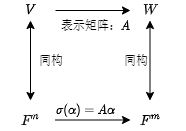
\includegraphics[scale=0.75]{./figs/6/6-1.png}
\end{figure}

图中我们可以看出通过坐标映射后得到的新映射即为定理4.1描述的映射.

在描述下一定理之前,我们首先介绍过渡矩阵(变换矩阵)的概念.
\begin{definition}
	设$B_1=\{\alpha_1,\alpha_2,\cdots,\alpha_n\}$与$B_2=\{\beta_1,\beta_2,\cdots,\beta_n\}$是线性空间
	$V(\mathbf{F})$的任意两组基,$B_2$中每个基向量被基$B_1$表示为
	$$\begin{cases}
		\beta_1=a_{11}\alpha_1+a_{21}\alpha_2+\cdots+a_{n1}\alpha_n \\
		\beta_2=a_{12}\alpha_1+a_{22}\alpha_2+\cdots+a_{n2}\alpha_n \\
		\cdots \\
		\beta_n=a_{1n}\alpha_1+a_{2n}\alpha_2+\cdots+a_{nn}\alpha_n
	\end{cases}.$$
	将上式用矩阵表示为
	$$(\beta_1,\beta_2,\cdots,\beta_n)=(\alpha_1,\alpha_2,\cdots,\alpha_n)\begin{pmatrix}
		a_{11} & a_{12} & \cdots & a_{1n} \\
		a_{21} & a_{22} & \cdots & a_{2n} \\
		\cdots & \cdots &        & \cdots \\
		a_{n1} & a_{n2} & \cdots & a_{nn}
	\end{pmatrix}.$$
	我们将这一矩阵称为即$B_1$变为基$B_2$的变换矩阵(或过渡矩阵).
\end{definition}
简单而言就是将$B_2$中的向量在$B_1$下的坐标按列排列.需要注意表述中是$B_1$变为基$B_2$还是反过来,
这两个矩阵互逆.注意过渡矩阵一定是基与基之间的表示矩阵,并且过渡矩阵一定可逆.
\begin{theorem}
	\textbf{基的选择对向量坐标的影响}
	
	设线性空间$V$的两组基为$B_1$和$B_2$,且基$B_1$到$B_2$的变换矩阵(过渡矩阵)为$A$,如果
	$\xi \in V(F)$,且在$B_1$和$B_2$下的坐标分别为$X$和$Y$,则$Y=A^{-1}X$.
\end{theorem}
上述即教材定理4.10,描述同一个向量在不同基下坐标之间的关系.事实上,这与本节同构关系紧密,因为
同构意味着两个线性空间结构一致,故同构映射可以保持向量组的线性关系不变.在同构关系下,
线性组合对应线性组合,线性无关对应线性无关,线性相关对应线性相关.我们有如下定理:
\begin{theorem}
	设$(\alpha_1,\alpha_2,\cdots,\alpha_n)$是线性无关的向量组,且
	$$(\beta_1,\beta_2,\cdots,\beta_s)=(\alpha_1,\alpha_2,\cdots,\alpha_n)A,$$
	则向量组$(\beta_1,\beta_2,\cdots,\beta_s)$的秩等于矩阵$A$的秩.
\end{theorem}
定理的证明需要用到坐标映射是同构映射这一事实,我们不难发现等式左侧向量组与$A$的列向量组是等价的.
事实上我们也可以由此发现,过渡矩阵一定是可逆矩阵.
\begin{theorem}
	已知$\beta_i=a_{1i}\alpha_1+a_{2i}\alpha_2+\cdots+a_{ni}\alpha_n(i=1,2,\cdots,n)$,
	且$A=(a_{ij})$可逆,则$\alpha_1,\alpha_2,\cdots,\alpha_n$与$\beta_1,\beta_2,\cdots,\beta_n$
	是等价的.
\end{theorem}
实际上这一定理与上一定理的思想都是类似的,我们可以看一个例题练习一下:
\begin{example}
	已知$\beta_1=\alpha_2+\alpha_3$,$\beta_2=\alpha_1+\alpha_3$,$\beta_3=\alpha_1+\alpha_2$,
	证明$\alpha_1,\alpha_2,\alpha_3$与$\beta_1,\beta_2,\beta_3$等价.
\end{example}
\begin{theorem}
	\textbf{基的选择对映射矩阵的影响}
	
	设线性变换$\sigma \in L(V,V)$,$B_1=\{\alpha_1,\dots,\alpha_n\}$和$B_2=\{\beta_1,\dots,\beta_n\}$
	是线性空间的$V(F)$的两组基,基$B_1$变为基$B_2$的变换矩阵为$C$,如果$\sigma$在基$B_1$下的矩阵为$A$,
	则$\sigma$关于基$B_2$所对应的矩阵为$C^{-1}AC$.
\end{theorem}
上述即教材定理7.4,研究同一个映射在不同基下表示矩阵之间的关系.实际上我们将在下一专题初等矩阵一节进一步讨论.
这一定理的证明需要用到我们之前描述的两种线性映射矩阵表示的统一性.

\vspace{2ex} 
\centerline{\heiti \Large 内容总结}

\vspace{2ex} 

\centerline{\heiti \Large 习题}
\vspace{2ex} 
{\kaishu }
\begin{flushright}
    \kaishu

\end{flushright}
\centerline{\heiti A组}
\begin{enumerate}
	\item 
\end{enumerate}
\centerline{\heiti B组}
\begin{enumerate}
	\item 
\end{enumerate}
\centerline{\heiti C组}
\begin{enumerate}
	\item 
\end{enumerate}
\chapter{线性映射的应用}

\section{线性空间的积}


\section{线性空间的商}


\section{对偶}


\vspace{2ex} 
\centerline{\heiti \Large 内容总结}

\vspace{2ex} 

\centerline{\heiti \Large 习题}
\vspace{2ex} 
{\kaishu }
\begin{flushright}
    \kaishu

\end{flushright}
\centerline{\heiti A组}
\begin{enumerate}
	\item 
\end{enumerate}
\centerline{\heiti B组}
\begin{enumerate}
	\item 
\end{enumerate}
\centerline{\heiti C组}
\begin{enumerate}
	\item 
\end{enumerate}
\chapter{矩阵基本运算}

\section{矩阵基本运算}
\subsection{基本概念}
\begin{enumerate}
    \item 矩阵的加法来源于线性映射的加法,矩阵相加要求两矩阵行列数一致,相加时只需对应位置元素相加即可;
    \item 矩阵的数乘来源于线性映射的数乘,计算只需矩阵的每个元素乘以常数即可;
    \item 矩阵的乘法来源于线性映射的复合,计算时要求前一个矩阵的列数等于后一个矩阵的行数,矩阵$A$与$B$
    相乘结果中第$i$行第$j$列元素为矩阵$A$的第$i$行与矩阵$B$的第$j$列对应位置元素相乘后求和的结果,
    即对于$A=(a_{ij})_{m \times n}$和$B=(b_{ij})_{n \times l}$,矩阵$C=AB=(c_{ij})_{m \times l}$,且
    $c_{ij}=a_{i1}b_{1j}+a_{i2}b_{2j}+\cdots+a_{in}b_{nj}\enspace(i=1,\ldots,m,\enspace j=1,\ldots,l)$.
\end{enumerate}

\subsection{基本性质}
\begin{enumerate}
    \item 回顾上一专题中$m \times n$矩阵构成的线性空间$\mathbf{M}_{m \times n}(\mathbf{F})$;
    \item 回顾矩阵乘法的基本性质:
    \begin{enumerate}[label=(\arabic*)]
        \item $(AB)C=A(BC)$(结合律)
        \item $\lambda(AB)=(\lambda A)B=A(\lambda B),\enspace \lambda \in \mathbf{F}$
        \item $A(B+C)=AB+AC$(左分配律)
        \item $(B+C)P=BP+CP$(右分配律)
        \item $A^kA^m=A^{k+m},\enspace (A^k)^m=A^{km}$,其中$A$为方阵,$k,m$为任意整数. 负整数对应于逆矩阵的情况.
    \end{enumerate}
    \item 回顾矩阵多项式的定义(利用线性映射多项式在基下的矩阵表示定义),
    并注意其交换性以及可因式分解性.
\end{enumerate}
\begin{example}
    展开矩阵多项式$(A+\lambda E)^n$.
\end{example}
\begin{example}
    设$f(x),g(x) \in \mathbf{F}[x],\enspace A,B \in \mathbf{M}_n(\mathbf{F})$. 证明:
    \[f(A)g(A)=g(A)f(A)\]
    \begin{enumerate}
        \item 如果$AB=BA$,则$f(A)g(B)=g(B)f(A)$;

        \item 设$f(x)=1+x+\cdots+x^{m-1}$,$g(x)=1-x$,$A=\begin{pmatrix}
            a & b \\ 0 & a
        \end{pmatrix}$,计算$f(A)g(A)$.
    \end{enumerate}
\end{example}
其他需要注意的性质:
\begin{enumerate}
    \item 矩阵乘法不一定满足交换律(即$AB$不一定等于$BA$).但是注意数量矩阵和任何矩阵相乘都是可交换的,因此求矩阵的幂次时,可以将其转化为$(A+\mu E)^n$(其中$E$为单位矩阵,$\mu$为常数)类型,然后利用二项式展开即可.很多情况下$A$都会是幂零矩阵,此时结果为有限项.
    \item $A\neq O$且$B\neq O$不能推出$AB\neq O$.例如线性方程组$AX = 0$有非零解,若$B$的各列均为方程非零解,则$AB = O$.
    \item 消去律也不一定满足:即$AB = AC$不一定$A = B$.原因在于$AB=AC \implies A(B-C)=O$,由(2)可知不一定$B = C$.
\end{enumerate}

\subsection{矩阵可交换问题}
一般来说在本课程中此类问题直接设可交换矩阵的每一个元素都是未知数即可,一些特殊的技巧
(使用关于一些特殊形状矩阵的结论)以及涉及到之后才能学到的知识的方法我们在这里也不展开了.我们只讨论一个基本的技巧,即
\[\forall t,\enspace AB=BA \iff (A-tE)B=B(A-tE)\]
此处的$t$根据矩阵的对角线上元素来决定,原则是使得其余矩阵与$A-tE$相乘的计算过程更为简单(一般是使得0元素更多),这样解方程也会更轻松.
我们来看一个简单的例子:
\begin{example}
    求与矩阵$A=\begin{pmatrix}
        3 & 0 & 0 \\ -1 & 3 & 0 \\ 0 & -1 & 3
    \end{pmatrix}$可交换的矩阵.
\end{example}

关于可交换我们有以下定理,证明并不是很复杂(教材习题中有出现):
\begin{theorem}
    \begin{enumerate}
        \item 与主对角元两两互异的对角矩阵可交换的方阵只能是对角矩阵;

        \item 准对角矩阵$A$每个对角分块内对角线元素相同,但不同对角块之间不同,则与$A$可交换的矩阵只能是准对角矩阵;

        \item 与所有$n$级可逆矩阵可交换的矩阵为数量矩阵;

        \item 与所有$n$级矩阵可交换的矩阵为数量矩阵.
    \end{enumerate}
\end{theorem}

\section{矩阵转置}
\subsection{基本概念}
实际上,矩阵的转置就是第$i$行变成了第$i$列,或者抽象表达为:
\[A=(a_{ij})_{m \times n},\enspace A^\mathrm{T}=(a'_{ji})_{n \times m},\enspace a_{ij}=a'_{ji}\]
写成矩阵形式就是:
\begin{definition}
    设$A=\begin{pmatrix}
        a_{11} & a_{12} & \cdots & a_{1n} \\
        a_{21} & a_{22} & \cdots & a_{2n} \\
        \vdots & \vdots & \ddots & \vdots \\
        a_{m1} & a_{m2} & \cdots & a_{mn}
    \end{pmatrix}$,称$\begin{pmatrix}
        a_{11} & a_{21} & \cdots & a_{m1} \\
        a_{12} & a_{22} & \cdots & a_{m2} \\
        \vdots & \vdots & \ddots & \vdots \\
        a_{1n} & a_{2n} & \cdots & a_{mn}
    \end{pmatrix}$为矩阵$A$的转置,记作$A^\mathrm{T}$.
\end{definition}

\subsection{基本性质}
\begin{enumerate}
    \item $(A^\mathrm{T})^\mathrm{T}=A$

    \item $(A+B)^\mathrm{T}=A^\mathrm{T}+B^\mathrm{T}$

    \item $(\lambda A)^\mathrm{T}=\lambda A^\mathrm{T},\enspace \lambda \in \mathbf{F}$

    \item $(AB)^\mathrm{T}=B^\mathrm{T}A^\mathrm{T}$,$(A_1A_2\cdots A_n)^\mathrm{T}=A_n^\mathrm{T}\cdots A_2^\mathrm{T}A_1^\mathrm{T}$

    \item $(A^\mathrm{T})^{-1}=(A^{-1})^\mathrm{T}$

    \item $(A^\mathrm{T})^m=(A^m)^\mathrm{T}$
\end{enumerate}

以上证明大都是平凡的,可以自己尝试完成.
\subsection{对阵矩阵与反对称矩阵}
\begin{definition}
    设$A=(a_{ij})_{n \times n}$,如果$\forall i,j=1,2,\ldots,n$均有$a_{ij}=a_{ji}$,
    则称$A$为对称矩阵. 若均有$a_{ij}=-a_{ji}$,则称$A$为反对称矩阵.
\end{definition}
易得$A$为对称矩阵的充要条件为$A=A^\mathrm{T}$,$A$为反对称矩阵的充要条件为$A=-A^\mathrm{T}$.
\begin{example}
    证明以下几点性质:
    \begin{enumerate}
        \item 反对称矩阵主对角元均为0;

        \item $AA^\mathrm{T}$和$A^\mathrm{T}A$均为对称矩阵;

        \item 设$A,B$为$n$阶对称和反对称矩阵,则$AB+BA$是反对称矩阵;

        \item 对称矩阵的乘积不一定对称;

        \item 可逆的对称(反对称)矩阵的逆矩阵也是对称(反对称)矩阵.
    \end{enumerate}
\end{example}

\section{初等矩阵}
\subsection{基本概念与性质}
\begin{definition}
    将单位矩阵$E$做一次初等变换得到的矩阵称为初等矩阵,与三种初等行、列变换对应的三类初等矩阵为:
    \begin{enumerate}
        \item 将单位矩阵第$i$行(或列)乘$c$,得到初等倍乘矩阵$E_i(c)$;

        \item 将单位矩阵第$i$行乘$c$加到第$j$行,或将第$j$列乘$c$加到第$i$列,得到初等倍加矩阵$E_{ij}(c)$;

        \item 将单位矩阵第$i,j$行(或列)对换,得到初等对换矩阵$E_{ij}$.
    \end{enumerate}
\end{definition}
请各位同学以矩阵形式写出以上三类矩阵.注意:
\begin{enumerate}
    \item 倍加变化请一定注意$i$和$j$在行列的情况下的不同;

    \item 三类矩阵不是三个矩阵,例如行列选择不唯一,常数选择不唯一;

    \item 注意三种初等矩阵都是可逆的,且$E_i^{-1}(c)=E_i\left(\dfrac{1}{c}\right)$,$E_{ij}^{-1}(c)=E_{ij}(-c)$,$E_{ij}^{-1}=E_{ij}$;

    \item 三种初等矩阵的转置:$E_i^\mathrm{T}(c)=E_i(c)$,$E_{ij}^\mathrm{T}(c)=E_{ji}(c)$,$E_{ij}^\mathrm{T}=E_{ij}$;
\end{enumerate}

初等矩阵大家非常关心为什么左乘代表行变换,右乘代表列变换.以右乘为例,我们来看矩阵$A$和$B$相乘的任一列结果.我们可以将矩阵$A$
按列做分块矩阵得到$\begin{pmatrix}\alpha_1,\ldots,\alpha_n\end{pmatrix}$,$\alpha_i$即表示$A$的第$i$列.然后矩阵$B$的第$j$列为列向量$(x_1,\ldots,x_n)^\mathrm{T}$,
由于矩阵$A$与$B$相乘结果第$j$列就是$A$与$B$的第$j$列相乘结果(回顾矩阵乘法的计算方式),则有$B$的第$i$列等于
$x_1\alpha_1+\cdots+x_n\alpha_n$即为$A$的全部列向量的线性组合,故右乘矩阵$A$得到矩阵的任一列都是$A$的全部列向量的线性组合,
所以右乘可以代表列变换.注意我这里并没有限制矩阵$B$为初等矩阵或可逆矩阵.

实际上左乘表示行变换可以用类似方法说明,只需按行对$B$分块即可.这一思想是特别重要的,在很多时候如果我们意识到左右乘是对被乘矩阵的行列
重新线性组合,思路会清晰很多.

关于初等矩阵还有一个相当重要的定理:

\begin{theorem}
    任意可逆矩阵都可以被表示为若干个初等矩阵的乘积.
\end{theorem}
定理证明只需要回忆高斯消元法可以将可逆矩阵化为单位矩阵即可.

利用矩阵初等变换我们可以获得本学期需要学习的三个矩阵标准形,因此这一内容虽然很基本但是非常重要:
\begin{enumerate}
    \item 相抵矩阵:本章已学习的内容,在之后会详细说明;
    \item 相似矩阵:若$P$为初等矩阵,对矩阵做$P^{-1}AP$变换即可得到与$A$相似的矩阵;
    \item 相合矩阵:两个矩阵,其中一个可以通过做相同的初等行列变换的到另一个矩阵(若$P$为初等矩阵,
    $P^{\mathrm{T}}AP$就是对$A$做了一次相同的初等行列变换).
\end{enumerate}
请同学们思考:如何从线性映射矩阵表示的角度理解初等变换与标准形的关系?在B组习题中将有练习进行体会
(实际上对矩阵表示的基做``初等变换''就是对表示矩阵做了初等变换,这两种变换行列方向不一致且矩阵互逆).

\section{矩阵的逆}
\subsection{基本概念}
\begin{definition}
    设$A \in \mathbf{M}_n(\mathbf{F})$. 若存在$B \in \mathbf{M}_n(\mathbf{F})$使得$AB=BA=E$,则称矩阵$A$可逆,
    并把$B$称为$A$的逆矩阵,记作 $ B = A^{-1} $.
\end{definition}
注意,逆矩阵定义基于方阵,非方阵没有上述逆矩阵.广义逆矩阵允许非方阵,但那是另一个定义,
我们不需要掌握.对于可逆矩阵,注意以下两个定理:
\begin{theorem}
    可逆矩阵$A$的逆矩阵唯一.
\end{theorem}
\begin{theorem}
    $AB=E \iff A$与$B$互为逆矩阵.
\end{theorem}
这两个定理的证明教材中有,特别注意唯一性的证明,反证法的思路一定要掌握,十分经典.
还需要强调的一点是,逆矩阵来源于逆映射.
\subsection{基本性质}
\begin{enumerate}
    \item 注意没有加法性质(请举出反例),对于数乘有$(\lambda A)^{-1}=\lambda^{-1}A^{-1}$;

    \item $(AB)^{-1}=B^{-1}A^{-1},\enspace (A_1A_2\cdots A_k)^{-1}=A_k^{-1}\cdots A_2^{-1}A_1^{-1}$;

    \item $(A^k)^{-1}=(A^{-1})^k,\enspace A^kA^m=A^{k+m},\enspace (A^k)^m=A^{km}$;

    \item 若$A$和$B$可逆,则$A\neq O$且$B\neq O$能推出$AB\neq O$,并且$A$可逆且$AB=O$可以推出$B=O$,除此之外还有消去律成立,即$A$则有$AB=AC \implies B=C$成立.
\end{enumerate}

还需要熟练掌握可逆矩阵的几个等价条件:
\begin{theorem}
    设$A \in \mathbf{M}_n{\mathbf{F}}$,则下列命题等价:
    \begin{enumerate}
        \item $A$可逆;

        \item $r(A)=n$;

        \item $A$的$n$个行(列)向量线性无关;

        \item 齐次线性方程组$AX=0$只有零解;

        \item $|A|\neq 0$.
    \end{enumerate}
\end{theorem}
\begin{example}
    已知矩阵 $A=\begin{pmatrix}a & b & c \\ d & e & f \\ h & x & y\end{pmatrix}$ 的逆是 $A^{-1}=\begin{pmatrix}-1 & -2 & -1 \\ 2 & 1 & 0 \\ 0 & -3 & -1\end{pmatrix}$,

$B=\begin{pmatrix}a-2b & b-3c & -c \\ d-2e & e-3f & -f \\ h-2x & x-3y & -y\end{pmatrix}$.求矩阵 $X$ 满足:

\[X+\left(B(A^TB^2)^{-1}A^T\right)^{-1}=X\left(A^2(B^TA)^{-1}B^T\right)^{-1}(A+B)\]
\end{example}

\subsection{逆矩阵的求解(基本方法)}
\begin{enumerate}
    \item 利用解线性方程组的方法:假设$AX=b$,使用高斯消元法求解;

    \item 利用初等矩阵的方法(初等行变换为常用方法).
\end{enumerate}

注意,基于初等变换的方法是非常重要的,我们很多时候不要被题目吓到去采用其他
偏门的方法,实际上很多时候拿到一个具体的矩阵求逆,使用的方法就是初等行变换.

\begin{example}
    用上述两种方法求矩阵$A=\begin{pmatrix}1 & -1 & 1 \\ 0 & 1 & 2 \\ 1 & 0 & 4\end{pmatrix}$的逆矩阵.
\end{example}

\subsection{矩阵方程}
\begin{enumerate}
    \item 考虑以下情形(其中出现的矩阵除$X$外均可逆,$X$不一定是列向量):
    \begin{enumerate}[label=(\arabic*)]
        \item $AX=B \implies X=A^{-1}B, \enspace XA=B \implies X=BA^{-1}$;
        \item $AXB=C \implies X=A^{-1}CB^{-1}$;
    \end{enumerate}
    \item 考虑以下情形:$AX=B$但$A$不可逆($X$不一定是列向量),直接高斯消元即可;
    \item 考虑以下求解方式的合理性:
    \begin{enumerate}[label=(\arabic*)]
        \item 若求$A^{-1}$,只需对$(A,E)$只做初等行变换,可以得到$(E,A^{-1})$;
        \item 若求$A^{-1}B$,只需对$(A,B)$只做初等行变换,可以得到$(E,A^{-1}B)$;
        \item 若求$BA^{-1}$,只需对$\begin{pmatrix}
            A \\ B
        \end{pmatrix}$只做初等列变换,可以得到$\begin{pmatrix}
            E \\ BA^{-1}
        \end{pmatrix}$;
        \item 对$\begin{pmatrix}
            A & E \\ E & O
        \end{pmatrix}$的前$n$行与$n$列做相同的行列变换,可以得到$\begin{pmatrix}
            P^\mathrm{T}AP & P^\mathrm{T} \\ P & O
        \end{pmatrix}$.
    \end{enumerate}
\end{enumerate}

\begin{example}
    设$A=\begin{pmatrix}1 & 0 & 0 \\ 1 & 1 & 0 \\ 1 & 1 & 1\end{pmatrix},\
    B=\begin{pmatrix}0 & 1 & 1 \\ 1 & 0 & 1 \\ 1 & 1 & 0\end{pmatrix}$,求矩阵$X$满足:
    \[AXA+BXB=AXB+BXA+A(A-B)\]
\end{example}

\vspace{2ex}
\centerline{\heiti \Large 内容总结}

\vspace{2ex}

\centerline{\heiti \Large 习题}
\vspace{2ex}
{\kaishu }
\begin{flushright}
    \kaishu

\end{flushright}
\centerline{\heiti A组}
\begin{enumerate}
    \item
\end{enumerate}
\centerline{\heiti B组}
\begin{enumerate}
    \item
\end{enumerate}
\centerline{\heiti C组}
\begin{enumerate}
    \item
\end{enumerate}

\chapter{矩阵运算进阶}

\section{特殊矩阵}

\section{分块矩阵}

\section{矩阵的幂}

\chapter{矩阵的秩}

\section{矩阵的秩}

\section{相抵标准形}

\section{秩不等式}
\chapter{行列式(I)}

\section{行列式的几种定义}
很多教材采用``逆序数''定义行列式(感兴趣的同学可以参考丘维声《高等代数》等教材),但是本教材未提及,因此
我们作为复习课也不展开描述.本教材使用公理化定义(使用一些规则描述)并讲解了
递归式定义(按行(列)展开).

\subsection{公理化定义}
\begin{definition} \label{def:11:公理化定义}
    数域$\mathbf{F}$上的一个$n$阶行列式是取值于$\mathbf{F}$的$n$个$n$维向量
    $\alpha_1,\alpha_2,\ldots,\alpha_n \in \mathbf{F}^n$的一个函数,且$\forall \alpha_i,\beta_i \in \mathbf{F}^n$
    和$\forall \lambda \in \mathbf{F}$,满足下列规则:
    \begin{enumerate}
        \item(齐性)$D(\alpha_1,\ldots,\lambda\alpha_i,\ldots,\alpha_n)=\lambda D(\alpha_1,\ldots,\alpha_i,\ldots,\alpha_n)$;

        \item(加性,与 1 合称线性性)

        $D(\alpha_1,\ldots,\alpha_i+\beta_i,\ldots,\alpha_n)=D(\alpha_1,\ldots,\alpha_i,\ldots,\alpha_n)+D(\alpha_1,\ldots,\beta_i,\ldots,\alpha_n)$;

        \item(反对称性)$D(\alpha_1,\ldots,\alpha_i,\ldots,\alpha_j,\ldots,\alpha_n)=-D(\alpha_1,\ldots,\alpha_j,\ldots,\alpha_i,\ldots,\alpha_n)$;

        \item(规范性)$D(e_1,e_2,\ldots,e_n)=1$.
    \end{enumerate}
\end{definition}
在公理化定义中,我们将行列式定义为一个满足特定的运算性质的从列向量组合到数的函数.
事实上,公理化定义从是逆序数定义可以推导出的行列式的运算性质,教材采用这种定义避开了繁琐的说明.
除此之外,我们不难看出公理化定义可以形象地理解为对$n$维空间中体积的定义,
对几何意义感兴趣的同学可以参考 \href{https://b23.tv/BV1ys411472E}{3b1b《线性代数的本质》系列视频}相关内容.
\begin{example} \label{ex:11:公理化定义}
    使用\autoref{def:11:公理化定义} 验证下述命题的正确性:
    \begin{enumerate}
        \item 若行列式有一列为零向量,则行列式的值等于0.

        \item 若行列式有两列元素相同,则行列式的值等于0.

        \item 若行列式有两列元素成比例,则行列式的值等于0.

        \item 对行列式做倍加列变换,行列式的值不变.

        \item 若$\alpha_1,\alpha_2,\ldots,\alpha_n$线性相关,则$D(\alpha_1,\alpha_2,\ldots,\alpha_n)=0$.
    \end{enumerate}
\end{example}

\begin{example} \label{ex:11:公理化定义2}
    设向量$\alpha_1,\alpha_2,\beta_1,\beta_2$为三维列向量,又$A=(\alpha_1,\alpha_2,\beta_1),B=(\alpha_1,\alpha_2,\beta_2)$,
    且$|A|=3$,$|B|=2$,求$|2A+3B|$.
\end{example}

\subsection{递归式定义}
首先需要回顾余子式和代数余子式的概念:
\begin{definition} \label{def:11:余子式}
    在$n$阶行列式$D=|a_{ij}|_{n \times n}$中,去掉元素$a_{ij}$所在的第$i$行和第$j$列的所有元素
    而得到的$n-1$阶行列式称为元素$a_{ij}$的\keyterm{余子式}[minor],记作$M_{ij}$,并把数$A_{ij}=(-1)^{i+j}M_{ij}$
    称为元素$a_{ij}$的\keyterm{代数余子式}[cofactor].
\end{definition}
注意,虽然余子式和代数余子式在名称中含有式,但实际上他们是一个值.实际上行列式也称为``式'',但这些``式''
只是形状上有个形式,实际上只是一个值.
\begin{example} \label{ex:11:cofactor}
    根据\autoref{def:11:余子式} 计算行列式$\begin{vmatrix}
        2 & 1 & 3 \\
        -1 & 0 & 2 \\
        1 & 5 & -2
    \end{vmatrix}$每个元素的余子式和代数余子式.
\end{example}

接下来我们便可以给出递归式定义:
\begin{definition} \label{def:11:递归式定义}
    设$D=|a_{ij}|_{n \times n}$,则
    \begin{gather}
        \label{eq:11:递归式定义1}
        D=\sum_{k=1}^{n}a_{kj}A_{kj}=a_{1j}A_{1j}+a_{2j}A_{2j}+\cdots+a_{nj}A_{nj} \quad j=1,2,\ldots,n \\
        \label{eq:11:递归式定义2}
        D=\sum_{k=1}^{n}a_{ik}A_{ik}=a_{i1}A_{i1}+a_{i2}A_{i2}+\cdots+a_{in}A_{in} \quad i=1,2,\ldots,n
    \end{gather}
\end{definition}
其中$A_{ij}$即为\autoref{def:11:余子式} 给出的代数余子式,\autoref{eq:11:递归式定义1} 称为$D$对第$j$列的展开式,\autoref{eq:11:递归式定义2} 称为$D$对第$i$行的展开式.这一定义与公理化定义的
等价性不难证明.事实上,这一定义被称为递归式定义的原因是显然的(如果在程序设计课程中已经学习过递归的概念),它使用$n-1$阶行列式定义$n$阶行列式,我们对任意$n$阶行列式
都可以递归展开到1阶,从而得到最终行列式计算结果.
\begin{example} \label{ex:11:递归式定义}
    利用\autoref{def:11:递归式定义} 计算\autoref{ex:11:cofactor} 中的行列式,可以行列展开均使用并在上述公式中选取不同$i$和$j$以熟悉\autoref*{def:11:递归式定义},并注意体会递归式定义的含义.
\end{example}

递归式定义有一个相关的结论如下:
\begin{theorem}
    $n$阶行列式$D=|a_{ij}|_{n \times n}$的某一行(列)元素与另一行(列)相应元素的代数余子式
    的乘积之和等于0,即
    \begin{gather}
        \label{eq:11:递归式定义3}
        \sum_{k=1}^{n}a_{kj}A_{ki}=a_{1j}A_{1i}+a_{2j}A_{2i}+\cdots+a_{nj}A_{ni}=0 \quad j \neq i \\
        \label{eq:11:递归式定义4}
        \sum_{k=1}^{n}a_{jk}A_{ik}=a_{j1}A_{i1}+a_{j2}A_{i2}+\cdots+a_{jn}A_{in}=0 \quad j \neq i
    \end{gather}
\end{theorem}
我们若将行列式第$j$列元素替换为第$i$列元素,那么上述\autoref{eq:11:递归式定义3} 根据\autoref{def:11:递归式定义} 就是在求替换后的行列式,
并且有两列元素相同的行列式为0,我们便可以轻松地证明\autoref*{eq:11:递归式定义3},同理也可证明\autoref*{eq:11:递归式定义4}. 同学们可能
对\crefrange*{eq:11:递归式定义1}{eq:11:递归式定义4} 式繁杂的下标感到陌生,因此安排了\crefrange*{ex:11:公理化定义2}{ex:11:递归式定义} 希望大家熟悉这些公式.
\begin{example} \label{ex:11:递归式定义2}
    对\autoref{ex:11:递归式定义} 中的矩阵验证\autoref{def:11:公理化定义} 的正确性.
\end{example}
这一节中行列式是按照一行(列)展开的,若按多行(列)展开则需要相应的 Laplace 定理,感兴趣的同学可以了解.
\subsection{行列式的常用性质}
设$A,B \in \mathbf{F}^{n \times n}$,$k \in \mathbf{F}$,则
\begin{enumerate}
    \item 一般情况下,$|A \pm B| \neq |A|\pm|B|$;

    \item $|kA|=k^n|A|$;

    \item $A$可逆$\iff |A| \neq 0$;

    \item 初等矩阵行列式(注意初等矩阵不分行列,左乘右乘区分初等行列变换):$|E_{ij}|=-1,\enspace |E_i(c)|=c,\enspace |E_{ij}(k)|=1$;

    \item 利用4中的结论可以得到$|A^\mathrm{T}|=|A|$:

    \item 利用4中的结论可以得到$|AB|=|A||B|$,$|A^k|=|A|^k$;

    \item 利用4中的结论(求出初等矩阵逆矩阵行列式)可以得到若$A$可逆,则$|A^{-1}|=|A|^{-1}$.
\end{enumerate}

以上性质都可以基于定义或上述其他性质得到,下面介绍的性质需要用到``打洞法''(分块矩阵初等变换)
来证明:

\begin{enumerate}
    \item $\begin{vmatrix}
        A & O \\ O & B
    \end{vmatrix} = \begin{vmatrix}
        A & O \\ C & B
    \end{vmatrix} = \begin{vmatrix}
        A & D \\ O & B
    \end{vmatrix} = |A||B|,\ \begin{vmatrix}
        O & A \\ B & C
    \end{vmatrix} = (-1)^{kr}|A||B|$;

    \item 当$A$可逆时,有$\begin{vmatrix}
        A & B \\ C & D
    \end{vmatrix} = |A||D-CA^{-1}B|$,当$D$可逆时,有
    $\begin{vmatrix}
        A & B \\ C & D
    \end{vmatrix} = |D||A-BD^{-1}C|$,当$B$可逆时,有
    $\begin{vmatrix}
        A & B \\ C & D
    \end{vmatrix} = (-1)^{mn}|B||C-DB^{-1}A|$,当$C$可逆时,有
    $\begin{vmatrix}
        A & B \\ C & D
    \end{vmatrix} = (-1)^{mn}|C||B-AC^{-1}D|$;

    \item 设$A$和$B$分别是$n \times m$和$m \times n$矩阵,则$|E_n \pm AB|=|E_m \pm BA|$,且
    $|\lambda E_n \pm AB|=\lambda^{n-m}|\lambda E_m \pm BA|(n \geqslant m)$.
\end{enumerate}

还有一部分由这些性质可以推导的其他性质将出现在C组习题中供参考.这部分主要是技巧性内容,可以选择性完成.

\section{行列式的基本运算}
本节内容按照往年经验不是考试重点,实际上行列式这章在往年单独出现的
频率较低,一般都在求解特征值或者作为判断可逆等情况下作为结论使用,但是我们仍然需要掌握基本的行列式计算方法,
至少教材中给出的例题需要熟悉.

一般而言行列式的计算方法有根据定义求解(包括逆序数定义(包括低阶行列式直接计算公式)、公理化定义和递归式定义(或 Laplace 定理))、
高斯消元法化为上三角矩阵求解、拆分法(大拆分法、小拆分法)求解、加边法(升阶法)求解、特殊行列式求解
(如``箭形''行列式,循环行列式,Vandermonde 行列式)、递推法求解、数学归纳法求解(这两种方法一般用于大对角形)、
打洞法求解以及利用特征值求解等,具体方法我们将在下一讲中作为拓展展开讲解.

事实上,范德蒙行列式有着广泛的应用,在此我们证明\autoref{thm:4:覆盖定理}的有限维情形作为一个例子:
\begin{example}\label{ex:11:行列式证明覆盖定理}
    设$V_1,V_2,\ldots,V_s$是有限维线性空间$V$的$s$个非平凡子空间,证明:$V$中至少存在一个向量
    不属于$V_1,V_2,\ldots,V_s$中的任何一个,即$V_1 \cup V_2 \cup \cdots \cup V_s\subsetneq V.$
\end{example}
\begin{proof}
    设$\dim V=n$,设$\vec{\alpha_1},\vec{\alpha_2},\cdots,\vec{\alpha_n}$为$V$的一组基,构造向量组$\{\vec{\beta_k}\}$中每个元素满足
    \[\vec{\beta_k}=\vec{\alpha_1}+k\vec{\alpha_2}+\cdots+k^{n-1}\alpha_n,k=1,2,3,\cdots\]
    任取上述向量组中的$n$个向量$\vec{\beta_{k_1}},\vec{\beta_{k_2}},\cdots,\vec{\beta_{k_n}}$,其中
    $k_1<k_2<\cdots<k_n$,则有
    \[(\vec{\beta_{k_1}},\vec{\beta_{k_2}},\cdots,\vec{\beta_{k_n}})=(\vec{\alpha_1},\vec{\alpha_2},\cdots,\vec{\alpha_n})C\]
    其中
    \[C=\begin{pmatrix}
        1 & 1 & \cdots & 1 \\
        k_1 & k_2 & \cdots & k_n \\
        \vdots & \vdots &  & \vdots \\
        k_1^{n-1} & k_2^{n-1} & \cdots & k_n^{n-1}
    \end{pmatrix}.\]
    则$|C|$是一个范德蒙行列式,由范德蒙行列式的性质可知$|C| \neq 0$,因此$C$可逆,又由于
    $\vec{\alpha_1},\vec{\alpha_2},\cdots,\vec{\alpha_n}$是$V$的一组基,因此
    $\vec{\beta_{k_1}},\vec{\beta_{k_2}},\cdots,\vec{\beta_{k_n}}$线性无关,从而
    向量组$\{\vec{\beta_k}\}$中任意$n$个向量均构成$V$的一组基.

    由于$V_1,V_2,\ldots,V_s$是$V$的非平凡子空间,因此每个子空间最多包含$\{\vec{\beta_k}\}$中$n-1$个向量,
    进而$V_1\cup V_2\cup\ldots\cup V_s$只包含$\{\vec{\beta_k}\}$中有限个向量,
    所以必然存在一个向量$\vec{\beta}_j$使得$\vec{\beta}_j \notin V_1\cup V_2\cup\ldots\cup V_s$.
\end{proof}

\section{伴随矩阵}
伴随矩阵是一个重要的概念,其性质都比较经典,而且往年也有考察.
\subsection{伴随矩阵的定义与性质}
\begin{definition}
    称矩阵$A^*=\begin{pmatrix}
        A_{11} & A_{21} & \cdots & A_{n1} \\
        A_{12} & A_{22} & \cdots & A_{n2} \\
        \vdots & \vdots & \ddots & \vdots \\
        A_{1n} & A_{2n} & \cdots & A_{nn}
    \end{pmatrix}$为$A$的\keyterm{伴随矩阵}[adjugate matrix],其中$A_{ij}$是元素$a_{ij}$的代数余子式.
\end{definition}
我们要特别注意伴随矩阵代数余子式的下标与通常矩阵下标不一致,与转置下标一致.
伴随矩阵具有以下几个重要性质,请各位同学掌握其证明并理解:
\begin{example} \label{ex:11:伴随矩阵}
    证明下列关于$n$阶矩阵$A$的伴随矩阵$A^*$的性质:
    \begin{enumerate}
        \item $AA^*=A^*A=|A|E$,若$A$可逆,则有$A^{-1}=|A|^{-1}A^*$,$A^*=|A|A^{-1}$,$(A^*)^{-1}=(A^{-1})^*=|A|^{-1}A$.

        \item $r(A^*)=\begin{cases}
        n & r(A)=n \\ 1 & r(A)=n-1 \\ 0 & r(A) < n-1
    \end{cases}$.

        \item $|A^*|=|A|^{n-1}$,无论$A$是否可逆.

        \item $(AB)^*=B^*A^*$,$(A^\mathrm{T})^*=(A^*)^\mathrm{T}$,$(kA)^*=k^{n-1}A^*$,要求掌握$A$可逆时的证明,
        若不可逆则需要使用第二节习题C组中对角占优的推论证明.

        \item $(A^*)^*=|A|^{n-2}A$,$|(A^*)^*|=|A|^{(n-1)^2}$,无论$A$是否可逆(本题结论可以推广到更多重的伴随矩阵).

        \item 对正整数$k$,$(A^k)^*=(A^*)^k$.
    \end{enumerate}
\end{example}

在计算行列式时若出现伴随矩阵,我们经常使用\autoref{ex:11:伴随矩阵} 中的1,3进行计算.

使用伴随矩阵求逆矩阵是一种矩阵求逆的方式,我们通过一个简单的例子复习伴随矩阵的基本定义和性质:
\begin{example}
    判断矩阵$\begin{pmatrix}
        1 & 2 & 3 \\ 2 & 1 & 2 \\ 1 & 3 & 3
    \end{pmatrix}$是否可逆. 若可逆,利用伴随矩阵求其逆矩阵.
\end{example}

\section{Cramer法则}
本节内容大家了解即可,要了解Cramer法则的内容及其与线性方程组的关系.教材中还有部分几何的内容,
感兴趣的同学可以了解,当然一般而言几何部分不会考察.
\subsection{Cramer法则}
\begin{theorem} \keyterm{Cramer法则} \label{thm:11:Cramer}
    对线性方程组
    \begin{gather}
        \label{eq:11:线性方程组1}
        \left\{ \begin{array}{rcl}
            a_{11}x_1+a_{12}x_2+\cdots+a_{1n}x_n&=&0 \\
            a_{21}x_1+a_{22}x_2+\cdots+a_{2n}x_n&=&0 \\
            &\vdots& \\
            a_{n1}x_1+a_{n2}x_2+\cdots+a_{nn}x_n&=&0
        \end{array} \right.
        \\
        \label{eq:11:线性方程组2}
        \left\{ \begin{array}{rcl}
            a_{11}x_1+a_{12}x_2+\cdots+a_{1n}x_n&=&b_1 \\
            a_{21}x_1+a_{22}x_2+\cdots+a_{2n}x_n&=&b_2 \\
            &\vdots& \\
            a_{n1}x_1+a_{n2}x_2+\cdots+a_{nn}x_n&=&b_n
        \end{array} \right.
    \end{gather}

    令$D=\begin{vmatrix}
        a_{11} & a_{12} & \cdots & a_{1n} \\
        a_{21} & a_{22} & \cdots & a_{2n} \\
        \vdots & \vdots & \ddots & \vdots \\
        a_{n1} & a_{n2} & \cdots & a_{nn}
    \end{vmatrix},D_1=\begin{vmatrix}
        b_1 & a_{12} & \cdots & a_{1n} \\
        b_2 & a_{22} & \cdots & a_{2n} \\
        \vdots & \vdots & \ddots & \vdots \\
        b_n & a_{n2} & \cdots & a_{nn}
    \end{vmatrix},\ldots,D_n=\begin{vmatrix}
        a_{11} & a_{12} & \cdots & b_1 \\
        a_{21} & a_{22} & \cdots & b_2 \\
        \vdots & \vdots & \ddots & \vdots \\
        a_{n1} & a_{n2} & \cdots & b_n
    \end{vmatrix}$,其中$D$称为系数行列式.
    \begin{enumerate}
        \item 方程组 \ref{eq:11:线性方程组1} 只有零解$\iff D \neq 0$,有非零解(无穷多解)$\iff D=0$,即$r(A)<n$;

        \item 方程组 \ref{eq:11:线性方程组2} 有唯一解$\iff D \neq 0$,此时$x_i=\dfrac{D_i}{D}\enspace(i=1,2,\ldots,n)$,
        当$D=0$时,方程组 \ref{eq:11:线性方程组2} 要么无解,要么有无穷多解.
    \end{enumerate}
\end{theorem}
我们可以用 Cramer 法则求解线性方程组,但要注意只有方程个数与未知数个数相等时才能使用,
并且需要系数行列式不为0.
\begin{example}
    求解方程组$\begin{cases}
        x_1+x_2+x_3=1 \\
        a_1x_1+a_2x_2+a_3x_3=0 \\
        a_1^2x_1+a_2^2x_2+a_3^2x_3=0
    \end{cases}$,其中$a_1,a_2,a_3$两两不等.
\end{example}

\section{行列式的秩}
\subsection{行列式的秩}
首先我们需要给出矩阵的子式、主子式的定义,然后给出相关的顺序主子式的定义.
\begin{definition}
    矩阵$A=(a_{ij})_{n \times n}$的任意$k$行($i_1<i_2<\cdots<i_k$行)和
    任意$k$列($j_1<j_2<\cdots<j_k$列)的交点上的$k^2$个元素排成的行列式
    \[\begin{vmatrix}
        a_{i_1j_1} & a_{i_1j_2} & \cdots & a_{i_1j_k} \\
        a_{i_2j_1} & a_{i_2j_2} & \cdots & a_{i_2j_k} \\
        \vdots & \vdots & \ddots  & \vdots \\
        a_{i_kj_1} & a_{i_kj_2} & \cdots & a_{i_kj_k}
    \end{vmatrix}\]
    称为矩阵$A$的一个$k$阶子式,若子式等于0则称$k$阶零子式,否则称非零子式.
    当$A$为方阵且$i_t=j_t\enspace(t=1,2,\ldots,k)$(即选取相同行列)时,称为$A$的
    $k$阶\keyterm{主子式}[principal minor]. 若$i_t=j_t=t\enspace(t=1,2,\ldots,k)$,称为$A$的$k$阶\keyterm{顺序主子式}[leading principal minor]
    (取前$k$行$k$列的左上角主子式).
\end{definition}
\begin{example}
    写出矩阵$\begin{pmatrix}
        1 & 5 & -2 \\ 2 & 3 & 4 \\ -1 & -3 & 0
    \end{pmatrix}$的所有一阶、二阶子式、主子式和顺序主子式.
\end{example}
接下来我们给出行列式的秩的定义.
\begin{definition}
    矩阵$A$的非零子式的最高阶数$r$称为$A$的行列式秩.
\end{definition}
\raggedright 其含义为$A$至少有一个$r$阶子式不为0,但所有$r+1$阶子式均为0.根据教材定理:
\begin{theorem}
    矩阵$A$的秩$r(A)=r \iff A$的行列式的秩为$r$.
\end{theorem}
\raggedright 我们可以得到上一个专题中矩阵的秩的等价定义.
\begin{definition}
    矩阵$A$的非零子式的最高阶数$r$称为矩阵$A$的秩,记为$r(A)$.
\end{definition}
\begin{example}
    利用定义求矩阵$\begin{pmatrix}
        1 & 1 & -1 & 3 \\ 1 & 2 & 1 & 1 \\ 2 & 3 & 0 & 4
    \end{pmatrix}$的行列式秩.
\end{example}
\subsection{关于秩的总结}
本学期我们一共学习了四个秩的概念:向量组的秩,线性映射的秩,矩阵的秩和行列式的秩.
事实上,我们在矩阵三秩相等性的证明中通过维数公式以及正交补等统一了向量组的秩(行秩、列秩的定义基于向量组的秩)
和线性映射的秩(矩阵的秩的定义基于线性映射的秩),在行列式一章中统一了矩阵的秩和行列式的秩
(利用行列式不为0与可逆的等价性). 至此我们统一了这四个秩,我们了解到虽然线性映射的秩、矩阵的秩、
行列式的秩的定义各不相同,但本质都在于向量组的秩(回顾线性映射的秩的定义,矩阵三秩相等以及行列式子式
不为0与矩阵可逆的关系,矩阵可逆与向量组的秩的关系). 这给我们的启示是上述提到的概念都可以互相转化考虑.
例如考虑可逆时,我们可以考虑行、列向量是否线性无关/矩阵对应的线性映射是否可逆/行列式是否为0等.
虽然说起来很简单,但是实际做题的时候很多同学还是容易思维局限,因此我们需要将这些概念的统一性放在重要的位置.

\vspace{2ex}
\centerline{\heiti \Large 内容总结}

\vspace{2ex}

\centerline{\heiti \Large 习题}
\vspace{2ex}
{\kaishu }
\begin{flushright}
    \kaishu

\end{flushright}
\centerline{\heiti A组}
\begin{enumerate}
    \item
\end{enumerate}
\centerline{\heiti B组}
\begin{enumerate}
    \item
\end{enumerate}
\centerline{\heiti C组}
\begin{enumerate}
    \item
\end{enumerate}

\chapter{行列式计算进阶}

\vspace{2ex}
\centerline{\heiti \Large 内容总结}

\vspace{2ex}

\centerline{\heiti \Large 习题}
\vspace{2ex}
{\kaishu }
\begin{flushright}
    \kaishu

\end{flushright}
\centerline{\heiti A组}
\begin{enumerate}
    \item
\end{enumerate}
\centerline{\heiti B组}
\begin{enumerate}
    \item
\end{enumerate}
\centerline{\heiti C组}
\begin{enumerate}
    \item
\end{enumerate}

\chapter{朝花夕拾}

\section{线性方程组解的一般理论}

\section{理论应用}

\section{线性方程组拓展题型}

\chapter{多项式}

\section{多项式的定义}

我们从多项式的定义开始.对于函数 $p:\mathbf{F}\to\mathbf{F}$,若存在
$a_0,\ldots,a_m\in\mathbf{F}$使得对任意$z\in\mathbf{F}$有
$p(z)=a_0+a_1z+\cdots+a_mz^m$,则称函数$p$为系数在$\mathbf{F}$中的多项式.

对于一个定义,我们很关心它是否能带来一些简便,系数的唯一性便是一个很好的使得研究简便的性质.
回顾之前证明一个向量在一组线性无关向量下的坐标唯一的证明,我们需要零向量在线性无关向量组
下的坐标为0这一条件.在多项式中,这一定理转变为
\begin{theorem}
    设$a_0,\ldots,a_m\in\mathbf{F}$,若对任意$z\in\mathbf{F}$有$a_0+a_1z+\cdots+a_mz^m=0$,
    则$a_0=\cdots=a_m=0$.
\end{theorem}
基于此我们可以得到多项式的系数必然唯一,否则两相等多项式之差为0却可以有非零系数.
(本质上将)$1,x,x^2,\ldots$视为多项式构成的线性空间的一组基即可)

\section{零点与因式}

接下来我们研究多项式的零点与因式,从而可以引出多项式的分解.
我们称$s\in\mathbf{F}[x]$为多项式$p\in\mathbf{F}[x]$的因式,如果
存在多项式$q\in\mathbf{F}[x]$使得$p=sq$.但很多时候并不能整除,因此我们需要引入
多项式的带余除法:
\begin{theorem}
    设$p,s\in\mathbf{F}[x]$且$s\neq 0$,则存在唯一的多项式$q,r\in\mathbf{F}[x]$,
    使得$p=sq+r$,且$\deg r<\deg s$.
\end{theorem}
这一定理实际上是数的带余除法的延伸,证明是基本的,可参考教材4.8.
\begin{example}
    设多项式$f(x)$被$(x-1),(x-2),(x-3)$除后,余式分别为$4,8,16$.求$f(x)$被$(x-1)(x-2)(x-3)$除后的余式.
\end{example}
基于此我们可以研究多项式零点和因式的性质:
\begin{theorem}
    设$p\in\mathbf{F}[x]$.
    \begin{enumerate}
        \item 若$\lambda\in\mathbf{F}$,则$p(\lambda)=0$当且仅当存在多项式
            $q\in\mathbf{F}[x]$使得对每个$z\in\mathbf{F}$均有$p(z)=(z-\lambda)q(z)$;

        \item 若$p$是$m\enspace(m \geqslant 0)$次多项式,则$p$在$\mathbf{F}$上最多有$m$个互不相等的零点.
    \end{enumerate}
\end{theorem}
1 的证明基于带余除法,2只需基于1即可,都非常基本.我们希望2的最多能够在复数域的情况下取到,
这需要接下来这一基本而伟大的定理——代数学基本定理作为支撑:
\begin{theorem} \textbf{\heiti 代数学基本定理} \label{thm:14:代数学基本定理}
    非常数复多项式在复平面上必有零点.
\end{theorem}

代数基本定理最简单直接的证明来源于复分析中的刘维尔定理或柯西积分公式,感兴趣的同学可以学习,
这里只需要承认这一定理.基于此我们可以进行多项式的分解,我们分复数域和实数域进行讨论:
\begin{theorem} \label{thm:14:多项式分解}
    设$p\in\mathbf{F}[x]$是非常数多项式,则$p$可以唯一分解(不计因式的次序)为
    \begin{enumerate}
        \item $(\mathbf{F}=\mathbf{C})\quad p(z)=c(z-\lambda_1)\cdots(z-\lambda_m)$,
        其中$c,\lambda_1,\ldots,\lambda_m\in\mathbf{C}$;

        \item $(\mathbf{F}=\mathbf{R})\quad p(x)=c(x-\lambda_1)\cdots(x-\lambda_m)
        (x^2+b_1x+c_1)\cdots(x^2+b_Mx+c_M)$,其中$c,\lambda_1,\ldots,\lambda_m,b_1,\ldots,b_M,
        c_1,\ldots,c_M\in\mathbf{R}$,并且对每个$j$均有$b_j^2<4c_j$.
    \end{enumerate}
\end{theorem}
1 的证明基于代数学基本定理是简单的,唯一性也较为显然. 2的证明需要教材4.15和4.16的支持,
剩余的证明也是基本的.
\begin{example}
    证明:每个奇数次的实系数多项式都有实的零点.
\end{example}
\begin{example}
    设$p\in\mathbf{F}[x]$且$q\neq 0$.证明:$c$是$f(x)$的$k\enspace(k\geqslant 1)$重根的充要条件为
    \[f(c)=f'(c)=\cdots=f^{(k-1)}(c),\enspace f^{(k)}(c)\neq 0.\]
\end{example}
除此之外需要提及的是,若上述定理中$c=1$,则多项式最高次数的项的系数为1,则称这一多项式为\keyterm{首一多项式}[monic polynomial].

\section{整除与互素}

提到因式我们很容易想到类似于整数的最大公因数的定义,这里我们依次引入整除、公因式和最大公因式的概念:
\begin{definition}
    设$p,q\in\mathbf{F}[x]$且$q\neq 0$,则$q$整除$p$或$p$能被$q$整除(记为$q \mid p$)当且仅当
    $p$除以$q$的余式为0.
\end{definition}
\begin{example}
    设$p,q\in\mathbf{F}[x]$,证明:$p^2 \mid q^2\iff p \mid q$.
\end{example}
\begin{definition}
    在$\mathbf{F}[x]$中,若$s \mid p$且$s \mid q$,则称$s$是$p$和$q$的一个公因式.若$p$和$q$的公因式$s$
    满足对$p$和$q$的任一公因式$s'$都有$s' \mid s$,则称$s$是$p$和$q$的一个最大公因式.
\end{definition}
故我们可以看出,当$p$和$q$不为0时,最大公因式即为次数最大的公因式.相应的,我们也有最小公倍式的定义,这也类似于
整数中的最小公倍数,我们不再赘述.

类似于整数中的辗转相除法(或称欧几里得算法),对于多项式我们有如下结论:
\begin{theorem}\label{thm:14:欧几里得算法}
    设$p,q\in\mathbf{F}[x]$,存在它们的一个最大公因式$s$,则存在$u,v\in\mathbf{F}[x]$
    使得\[s=up+vq.\]
\end{theorem}
证明与欧几里得算法的构造是类似的,感兴趣的同学可以回顾初等数论的知识.在本节中我们更重视$p,q$最大公因式
为1的情况,我们称之为\keyterm{互素}[coprime],我们可以得到一个多项式互素的充要条件:
\begin{theorem}\label{thm:14:裴蜀定理}
    设$p,q\in\mathbf{F}[x]$,则$p$和$q$互素的充要条件是存在$u,v\in\mathbf{F}[x]$
    使得\[up+vq=1.\]
\end{theorem}
这一定理称之为\keyterm{裴蜀定理}[B\'ezout's Lemma],必要性根据\autoref{thm:14:欧几里得算法} 可以直接得到,充分性可以设$p$和$q$
的公因式为$s$,于是等式两边可以同时约去$s$,这表明必有$s \mid 1$,故$s=1$,$p,q$必然互素.
\begin{example}
    证明:$\mathbf{F}[x]$中两个次数大于0的多项式没有公共复根的充要条件是它们互素.
\end{example}

\vspace{2ex}
\centerline{\heiti \Large 内容总结}

\vspace{2ex}

\centerline{\heiti \Large 习题}
\vspace{2ex}
{\kaishu }
\begin{flushright}
    \kaishu

\end{flushright}
\centerline{\heiti A组}
\begin{enumerate}
    \item
\end{enumerate}
\centerline{\heiti B组}
\begin{enumerate}
    \item
\end{enumerate}
\centerline{\heiti C组}
\begin{enumerate}
    \item
\end{enumerate}

\chapter{不变子空间}

\section{不变子空间的定义}

\section{特征值与特征多项式}

\section{特征向量与特征子空间}

\vspace{2ex} 
\centerline{\heiti \Large 内容总结}

\vspace{2ex} 

\centerline{\heiti \Large 习题}
\vspace{2ex} 
{\kaishu }
\begin{flushright}
    \kaishu

\end{flushright}
\centerline{\heiti A组}
\begin{enumerate}
	\item 
\end{enumerate}
\centerline{\heiti B组}
\begin{enumerate}
	\item 
\end{enumerate}
\centerline{\heiti C组}
\begin{enumerate}
	\item 
\end{enumerate}
\chapter{相似标准形}

\section{上三角矩阵}

\section{对角矩阵}

\section{分块对角矩阵}

\chapter{多项式的进一步讨论}

\section{特征多项式 \quad Hamilton-Cayley 定理}
接下来的内容我们希望讨论一类特殊的多项式,将算子代入后多项式值为0. 这样的多项式我们称为算子的
零化多项式,讨论这一内容可以让我们从其他角度进一步理解矩阵标准形.
\begin{definition}
    设$T\in \mathcal{L}(V)$,若$p\in\mathbf{F}[x]$使得$p(T)=0$,则称$p$为$T$的一个\keyterm{零化多项式}[annihilating polynomial].
\end{definition}
矩阵的零化多项式有类似的定义(后面多项式都有类似的定义,将算子替换为矩阵即可,并且基于算子的定理都可以推广到算子
对应的矩阵). 接下来我们讨论一类多项式,我们在第六章实际上已经提到过,但我们这里给出一种新的理解:
\begin{definition}
    设$V$是复向量空间,$T\in \mathcal{L}(V)$.令$\lambda_1,\ldots,\lambda_m$表示$T$的所有互异本征值,
    重数分别为$d_1,\ldots,d_m$,则多项式\[(z-\lambda_1)^{d_1}\cdots(z-\lambda_m)^{d_m}\]
    称为$T$的\keyterm{特征多项式}[characteristic polynomial].
\end{definition}
根据这一定义,$T$的特征多项式的次数为$\dim V$(由\autoref{th:16:gen-eigen} (2) 可得), % TODO 引用
并且其零点恰为$T$的全部本征值.回忆定理\ref{特征多项式1}对特征多项式的定义,$f(\lambda)=|\lambda I-A|$,
且多项式的$k$重根即为$k$重本征值,本征值的重数也就称为代数重数.
\begin{example}
    设$V$是复向量空间,$V_1,\cdots,V_m$都是$V$的非零子空间使得$V=V_1\oplus\cdots\oplus V_m$.设$T\in \mathcal{L}(V)$,每个
    $V_j$在$T$下不变.对每个$j$,令$p_j$表示$T|_{V_j}$的多项式.证明:$T$的特征多项式为$p_1\cdots p_m$.
\end{example}
实际上,根据\autoref{th:14:factorization-of-polynomial},我们知道这两个特征多项式的定义统一等价于两个代数重数的定义统一.教材在
10.25中直接证明了特征多项式的统一,然后我们可以得出代数重数定义统一,即广义本征空间重数等于本征值作为特征多项式
$|\lambda I-A|=0$的零点重数.

在上面的讨论中我们依据广义本征空间的维数定义特征多项式,接下来我们希望变换思路,利用第六章中的特征多项式的定义
推导广义本征空间的相关结论,这一正一逆的思路在某种程度上也体现出两个研究体系的等价性.

下面我们引入 Hamilton-Cayley 定理. 我们的动机是获得零化多项式. 观察矩阵$A=\begin{pmatrix}
    1 & 2 \\ 0 & -1
\end{pmatrix}$,我们容易验证$A^2-I=0$,因此$\lambda^2-1$是$A$的一个零化多项式,同时我们发现这是
$A$的特征多项式,因此我们可以猜想,是否对于所有的矩阵都有特征多项式是零化多项式的结论,事实上,这就是
著名的 \keyterm{Hamilton-Cayley 定理}:
\begin{theorem} \label{th:17:HC}
    设$V$是复向量空间,$T\in \mathcal{L}(V)$.令$q$表示$T$的特征多项式,则$q(T)=0$.
\end{theorem}
基于 Done Right 的体系,我们可以很轻松地利用广义本征空间分解证明这一定理.一般的高等代数教材引入$\lambda$矩阵
等不直观的方式证明,十分繁杂,这也体现了 Done Right 这一思路的优越性.

这一定理在解题时可能的应用在于求解一些矩阵多项式/求矩阵的逆/求矩阵的幂,都是偏向于技术性的,因此我们不在此展开.

接下来我们利用这一定理继续我们逆向推导的过程.我们的目标同样是找到能在直和后得到原空间
的不变子空间的定义方式.实际上我们可以参照以下结论:
\begin{theorem} \label{th:17:fact-and-direct-sum} % 多项式分解与零空间直和
    设$T\in \mathcal{L}(V)$,且在$\mathbf{F}[x]$中有$p=p_1p_2$,且$p_1,p_2$互素,则有
    \[\ker p(T)=\ker p_1(T)\oplus\ker p_2(T).\]
\end{theorem}
定理的证明我们留作习题,需要基于\autoref{th:14:bezout-lemma}. 我们需要将这一定理推广到因式更多的情况,
证明只需要依照\autoref{th:17:fact-and-direct-sum} 然后进行数学归纳法即可:
\begin{theorem} \label{th:17:fact-and-direct-sum-general}
    设$T\in \mathcal{L}(V)$,且在$\mathbf{F}[x]$中有$p=p_1p_2\cdots p_s$,且$p_1,p_2,\ldots,p_s$两两互素,
    则有\[\ker p(T)=\ker p_1(T)\oplus\ker p_2(T)\oplus\cdots\oplus\ker p_s(T).\]
\end{theorem}
这一定理表明,将多项式分解为互素的多项式乘积,原多项式作用于算子的零空间等于分解后各个互素因式作用于算子的零空间的直和.
我们结合 Hamilton-Cayley 定理,如果$p$是$T$的特征多项式,故$p(T)=0$,则$\ker p(T)$就是全空间$V$.接下来我们对第六章中
定义的特征多项式分解为互素因式乘积,有
\[p(\lambda)=|\lambda I-A|=(\lambda-\lambda_1)^{r_1}(\lambda-\lambda_2)^{r_2}\cdots(\lambda-\lambda_m)^{r_m},\]
其中$A$为$T$在某组基下的矩阵.能进行这样的分解的原因在于第六章中结论告诉我们特征多项式是首一的,且零点就是算子本征值,
根据\autoref{th:14:factorization-of-polynomial} 可以知道这样的分解存在且$\lambda_1,\ldots,\lambda_m$为$T$的所有互异本征值,$r_1,\ldots,r_m$为本征值
作为特征多项式零点的重数. 然后由于分解的因式显然是两两互素的,因此根据\autoref{th:17:fact-and-direct-sum-general},我们有
\[\ker p(T)=V=\ker (T-\lambda_1I)^{r_1}\oplus\cdots\oplus\ker (T-\lambda_mI)^{r_m},\]
这或许就是一种巧合,我们从多项式的角度也推导出了和广义本征空间相近的结论,并且这里将广义本征空间定义中$(T-\lambda I)$的幂次
降低了.除此之外,$\ker (T-\lambda_iI)^{r_i}\enspace(i=1,2,\ldots,m)$也是$T$的不变子空间,因此我们也能得到分块对角矩阵的标准形,
并且\autoref{th:16:gen-eigen} 的其他结论也可以基于此得到,此处不再赘述.

总结一下上述两种推导思路,其核心都在于寻找合适的不变子空间的直和分解,使得算子在直和分解获得的基下的矩阵是分块对角矩阵.
 Done Right 的思想基于从本征空间到广义本征空间的自然扩张(基本原理是零空间增长),这保持了不变子空间的性质并且使得所有算子
都有这样的直和分解,由此进一步得到 Hamilton-Cayley 定理.一般高等代数的思想在于首先引入$\lambda$矩阵理论得到 Hamilton-Cayley 定理,
然后基于\autoref{th:17:fact-and-direct-sum-general} 的直和分解得到合适的不变子空间直和分解.我们可以看出,Done Right 的思路相对而言更加直观,但其缺陷
也是显然的,很多具象的结论以及计算方式都在一般高等代数的思路中相对更为直接.所以 Done Right 向我们展示了高等代数中核心结论如何用更
符合直觉的方式得到,实际应用时原先等价的技术手段很多时候仍是不可或缺的.
\begin{example}
    设$T\in \mathcal{L}(V)$,$p(z)=a_nx^n+\cdots+a_1x\in\mathbf{F}[x]$是$T$的一个零化多项式,其中$a_1\neq 0$,证明:
    \[V=\ker T\oplus\textup{range }T.\]
\end{example}
下面我们希望将广义本征空间定义中$(T-\lambda I)$的幂次进一步降低到下界(即找到最低的幂次使得零空间停止增长),这需要引入极小多项式
的概念.

\section{极小多项式及其性质}
\begin{definition}
    设$T\in \mathcal{L}(V)$,则$T$的极小多项式是唯一一个使得$p(T)=0$的次数最小的首一多项式.
\end{definition}
这一定义的合理性需要下述定理保证:
\begin{theorem}
    设$T\in \mathcal{L}(V)$,则存在唯一一个次数最小的首一多项式$p$使得$p(T)=0$.
\end{theorem}
事实上,根据$1,T,T^2,\ldots,T^{(\dim V)^2}$的线性相关性(因为$\mathcal{L}(V)$空间是$(\dim V)^2$维的)可以知道极小多项式的最低次数最多为
$(\dim V)^2$,这一点早在第二章中就有涉及.而根据 Hamilton-Cayley 定理,特征多项式$p$是$\dim V$次的且$p(T)=0$,故极小多项式的最高次数的
上界进一步下降到$\dim V$.以上讨论都可以证明上述定理的存在性,唯一性的证明只需利用基于多项式带余除法的套路即可(这种基于次数的唯一性
证明是常见的,请务必掌握).

如果需要计算极小多项式,我们可以给出一个算法化的描述. 对于$m=1,2,\ldots$,我们相继考虑线性方程组
\[a_0M(I)+a_1M(T)+\cdots+a_{m-1}M(T^{m-1})+M(T^m)=0,\]
直到这一方程组有一个解$a_0,a_1,\ldots,a_{m-1}$,此时$a_0,a_1,\ldots,a_{m-1},1$即为极小多项式的次数.
\begin{example} \label{ex:17:minimal-poly}
    求矩阵$A=\begin{pmatrix}
        0 & 0 & 0 \\ 1 & 0 & 2 \\ 2 & 1 & -1
    \end{pmatrix}$和$B=\begin{pmatrix}
        2 & 2 & 1 \\ 0 & 2 & -1 \\ 0 & 0 & -3
    \end{pmatrix}$的最小多项式.
\end{example}
下面我们给出一些简单算子/矩阵的极小多项式:

\begin{enumerate}
    \item 幂零算子:$N\in \mathcal{L}(V)$且$N^l=0$,但$N^{l-1}\neq 0$($l$称为幂零指数),极小多项式为$\lambda^l$;

    \item 幂等算子:$T\in \mathcal{L}(V)$且$T^2=T$,极小多项式为$\lambda^2-\lambda$或$\lambda$或$\lambda-1$;

    \item 对合算子:$T\in \mathcal{L}(V)$且$T^2=I$,极小多项式为$\lambda^2-1$或$\lambda+1$或$\lambda-1$;

    \item 引入\keyterm{若当块}. 若域$\mathbf{F}$上的一个$r$级矩阵形如\[\begin{pmatrix}
        a & 1 & 0 & \cdots & 0 & 0 \\
        0 & a & 1 & \cdots & 0 & 0 \\
        \vdots & \vdots & \vdots & \ddots & \vdots & \vdots \\
        0 & 0 & 0 & \cdots & a & 1 \\
        0 & 0 & 0 & \cdots & 0 & a
    \end{pmatrix}\]
    则称其为一个$r$级若当块(1级显然就是1阶矩阵),记作$J_r(a)$,其中$a$是对角线上元素.不难得到其
    极小多项式等于特征多项式$(\lambda-a)^r$.
\end{enumerate}

我们利用多项式的带余除法以及 Hamilton-Cayley 定理可以得到下述简单的结论:
\begin{theorem}
    设$T\in \mathcal{L}(V)$.
    \begin{enumerate}
        \item $q\in\mathbf{F}[x]$,则$q(T)=0$当且仅当$q$是$T$的极小多项式的多项式倍;

        \item 设$\mathbf{F}=\mathbf{C}$,则$T$的特征多项式是$T$的极小多项式的多项式倍.
    \end{enumerate}
\end{theorem}
在\autoref{ex:17:minimal-poly} 中我们不难发现,两个矩阵的极小多项式和特征多项式根一致,实际上这是对任意算子(或矩阵)
都成立的结论:
\begin{theorem} \label{min-chr-same-root} % 极小与特征根相同
    设$T\in \mathcal{L}(V)$,则$T$的极小多项式的零点恰好是$T$的本征值,即极小多项式与特征多项式在$\mathbf{F}$中有
    相同的根(重数可以不同).
\end{theorem}
证明这一定理注意要证明两个方向,其一是极小多项式的零点都是特征多项式的零点,这只需要基于特征多项式是极小多项式的倍式;
另一方面是特征多项式的零点(本征值)都是极小多项式的零点,这也是简单的,只需要利用极小多项式是零化多项式以及本征值的基本性质即可.

这一定理是非常重要的,它关系到下一小节关于多项式和标准形关系的讨论.并且\autoref{ex:17:minimal-poly} 也可以基于此有更快的解法.
除此之外,我们还可以得到一个推论,即相似的矩阵有相同的极小多项式.因为上面的结论基于算子,相似矩阵对应的算子是一致的.

\section{多项式与标准形的应用}
在最后一小节我们尝试将两种描述算子的角度(标准形和多项式)联系起来,主要的桥梁就是上一小节中讨论的极小多项式.在前文讨论
特征多项式诱导的不变子空间分解时,我们将广义本征空间定义中需要求零空间的算子幂次降低,而依据\autoref{min-chr-same-root} 以及
特征多项式是极小多项式的倍式可知,这一幂次还可以进一步降低:
\begin{theorem} \label{th:17:decomp} % 极小多项式与分解
    设$T\in \mathcal{L}(V)$,$T$的极小多项式为$p=(\lambda-\lambda_1)^{s_1}\cdots(\lambda-\lambda_m)^{s_m}$,则有
    \[\ker p(T)=V=\ker (T-\lambda_1I)^{s_1}\oplus\cdots\oplus\ker (T-\lambda_mI)^{s_m}.\]
\end{theorem}
并且我们知道,极小多项式的因式次数无法继续降低,否则不为零化多项式,因此它也给出了广义本征空间定义中需要求零空间的算子的幂次为
何值时,零空间会停止增长,并且这是一个下界,基于此我们更进一步地理解了极小多项式因式次数的含义.

实际上我们也可以逆向思考,如果我们已知空间的不变子空间分解,我们应当如何求解极小多项式.实际上这一结论是很直观的,答案是各个不变子空间
的极小多项式的最小公倍式.证明我们留作习题,基本思想是利用限制算子说明全空间上的极小多项式是各个不变子空间的极小多项式的倍式.
这一结论的应用或许并不直接,但如果我们考虑算子在不变子空间直和分解下的分块对角矩阵,那么这一分块对角矩阵的极小多项式实际上就等于
各个分块的极小多项式的最小公倍式.
\begin{example} \label{th:17:jordan-min-poly} % 若当形矩阵极小多项式
    我们在此继续引入\keyterm{若当形矩阵},即由若干个若当块组成的分块对角矩阵. 设$A$为若当形矩阵,
    $A=\diag(J_{r_1}(a),\ldots,J_{r_s}(a),J_{t_1}(b),\ldots,J_{t_m}(b))$,其中$r_1\leqslant\cdots\leqslant r_s$,
    $t_1\leqslant\cdots\leqslant t_m$,则$A$的极小多项式$p$为$(\lambda-a)^{r_1},\ldots,(\lambda-a)^{r_s},(\lambda-b)^{t_1},(\lambda-b)^{t_m}$
    的最小公倍式,即为$(\lambda-a)^{r_s}(\lambda-b)^{t_m}$.实际上,这一结论还可以进一步推广,但描述较为繁杂,读者只需从此例理解基本思想即可.
\end{example}
在\autoref{th:17:decomp} 中我们了解了极小多项式中因子幂次与广义本征空间的关联.加入极小多项式的各个因式的次数均为1,这与可对角化算子的不变子空间
分解是一致的!因此我们可以得到下面的结论:
\begin{theorem}
    设$T\in \mathcal{L}(V)$,$T$可对角化当且仅当$T$的极小多项式能分解成不同的一次因式的乘积.
\end{theorem}
这给出了算子可对角化的另一等价条件,基于此,第六章中给出矩阵多项式判断可对角化的习题都可以``秒杀'',例如幂等矩阵、对合矩阵可对角化,但幂零矩阵除非自身
为0否则一定不可对角化,高于1阶的若当块矩阵一定不可对角化,包含高于1阶的若当块矩阵的若当形矩阵也一定不可对角化.

我们也可从矩阵的角度来理解.例如幂等矩阵$A$满足$A^2=A$,根据多项式诱导的不变子空间分解,我们很容易得到$A$为幂等矩阵的充要条件为$r(A)+r(A-E)=n$,
其它对合矩阵等情况各位同学也可以自己写出等价条件,虽然形式上可以千变万化,但实质就是多项式诱导的不变子空间分解.

除此之外,联系多项式互素分解与不变子空间分解的对应关系,这也表明算子可对角化当且仅当其各个广义本征空间就是其本征空间,即满足代数重数等于几何重数.
或者说$T$的每个广义本征向量都是其本征向量.
\begin{example}
    设$T\in \mathcal{L}(V)$,若$T$可对角化,则对于$T$的任意非平凡不变子空间$U$,都有$T\vert_U$可对角化.
\end{example}
\begin{example}
    已知某个实对称矩阵$A$的特征多项式为$\lambda^5+3\lambda^4-6\lambda^3-10\lambda^2+21\lambda-9$,求$A$的极小多项式.
\end{example}
\begin{example}
    设$V$为$n$阶方阵构成的线性空间,$T\in \mathcal{L}(V)$,$\forall A\in V, T(A)=2A-3A^{\mathrm{T}}$.
    \begin{enumerate}
        \item 求$T$的特征值;

        \item 证明:$T$可对角化.
    \end{enumerate}
\end{example}
我们需要补充说明一点,虽然矩阵相似不随数域改变而改变,但可对角化与数域有关.例如实矩阵$A$的极小多项式为$\lambda^3-1$,在它在实数域上无法分解为互素
一次因式的乘积,复数域上则可以,这表明$A$在实数域上不可对角化,但在复数域上可以.

\vspace{2ex}
\centerline{\heiti \Large 内容总结}

\vspace{2ex}

\centerline{\heiti \Large 习题}
\vspace{2ex}
{\kaishu }
\begin{flushright}
    \kaishu

\end{flushright}
\centerline{\heiti A组}
\begin{enumerate}
    \item
\end{enumerate}
\centerline{\heiti B组}
\begin{enumerate}
    \item
\end{enumerate}
\centerline{\heiti C组}
\begin{enumerate}
    \item
\end{enumerate}

\chapter{若当标准形}

\section{若当标准形的存在}

\section{若当标准形的求法}

\section{若当标准形的应用}
\chapter{内积空间}

\section{内积和范数}

\section{标准正交基}

\section{正交补}

\chapter{内积空间上的算子(I)}

\section{正交矩阵和酉矩阵}

\section{正定矩阵}

\vspace{2ex} 
\centerline{\heiti \Large 内容总结}

\vspace{2ex} 

\centerline{\heiti \Large 习题}
\vspace{2ex} 
{\kaishu }
\begin{flushright}
    \kaishu

\end{flushright}
\centerline{\heiti A组}
\begin{enumerate}
	\item 
\end{enumerate}
\centerline{\heiti B组}
\begin{enumerate}
	\item 
\end{enumerate}
\centerline{\heiti C组}
\begin{enumerate}
	\item 
\end{enumerate}
\chapter{内积空间上的算子(II)}

\section{自伴算子和正规算子}

\section{谱定理}

\chapter{二次型}

\section{双线性函数}

\section{二次型的标准形}

\section{惯性定理}

\vspace{2ex} 
\centerline{\heiti \Large 内容总结}

\vspace{2ex} 

\centerline{\heiti \Large 习题}
\vspace{2ex} 
{\kaishu }
\begin{flushright}
    \kaishu

\end{flushright}
\centerline{\heiti A组}
\begin{enumerate}
	\item 
\end{enumerate}
\centerline{\heiti B组}
\begin{enumerate}
	\item 
\end{enumerate}
\centerline{\heiti C组}
\begin{enumerate}
	\item 
\end{enumerate}
\chapter{极分解与奇异值分解}

\vspace{2ex}
\centerline{\heiti \Large 内容总结}

\vspace{2ex}

\centerline{\heiti \Large 习题}
\vspace{2ex}
{\kaishu }
\begin{flushright}
    \kaishu

\end{flushright}
\centerline{\heiti A组}
\begin{enumerate}
    \item
\end{enumerate}
\centerline{\heiti B组}
\begin{enumerate}
    \item
\end{enumerate}
\centerline{\heiti C组}
\begin{enumerate}
    \item
\end{enumerate}

\chapter{实空间上的算子}

\vspace{2ex} 
\centerline{\heiti \Large 内容总结}

\vspace{2ex} 

\centerline{\heiti \Large 习题}
\vspace{2ex} 
{\kaishu }
\begin{flushright}
    \kaishu

\end{flushright}
\centerline{\heiti A组}
\begin{enumerate}
	\item 
\end{enumerate}
\centerline{\heiti B组}
\begin{enumerate}
	\item 
\end{enumerate}
\centerline{\heiti C组}
\begin{enumerate}
	\item 
\end{enumerate}
\chapter{行列式(II)}

\vspace{2ex}
\centerline{\heiti \Large 内容总结}

\vspace{2ex}

\centerline{\heiti \Large 习题}
\vspace{2ex}
{\kaishu }
\begin{flushright}
    \kaishu

\end{flushright}
\centerline{\heiti A组}
\begin{enumerate}
    \item
\end{enumerate}
\centerline{\heiti B组}
\begin{enumerate}
    \item
\end{enumerate}
\centerline{\heiti C组}
\begin{enumerate}
    \item
\end{enumerate}

\chapter{线性代数与解析几何基础}

解析几何很大程度上是线性代数发展的初衷,在研究点线面以及几何体时,将集体的几何问题抽象化为代数问题使其方便解决与计算,即是解析几何的主要思想.
本节我们将会从线性代数的角度探究解析几何的一些基本概念与方法.此在线性代数课程的考察中也会有少部分的解析几何内容,但内容较浅,主要考察点、直线、平面等之间的关系.
\section{欧几里得空间}
在前面的学习中我们已经较为全面地学习了内积空间的相关知识,而在解析几何中,我们在更多情况下会研究\keyterm{欧几里得空间}[Euclidean Space]下的问题.
\begin{definition}[欧几里得空间]
    欧几里得空间(欧氏空间)是一个有限维实内积空间.
\end{definition}
同学们可能对欧氏空间的几何直观更为熟悉.当欧氏空间的维数为$2$或$3$时,我们可以用熟悉的平面直角坐标系与空间直角坐标系来描述欧氏空间中的向量,并用点积作为向量的内积.
\section{欧氏空间上的运算}
我们也已经基本掌握了模、内积、夹角等在内积空间中的基本概念,在此我们引入一些在先前的学习中接触较少的概念.
\begin{definition}
    \keyterm{点积}[dot product]是在三维欧氏空间中对两个向量的运算,用$\vec{a}\cdot\vec{b}$表示.两向量点积得到的数值等于两向量模长的乘积与两向量夹角的余弦的乘积.
\end{definition}
特别的,三维欧氏空间中的向量点积$(a_1,a_2,a_3)\cdot(b_1,b_2,b_3)$可以表示为$$a_1b_1+a_2b_2+a_3b_3$$
由点积的计算,我们可以很方便地得到两向量夹角的余弦,即$$\cos\theta=\frac{\vec{a}\cdot\vec{b}}{|\vec{a}||\vec{b}|}$$
\begin{definition}
    \keyterm{叉乘}[cross product]是在三维欧氏空间中对两个向量的运算,用$\vec{a}\times\vec{b}$表示.两向量叉乘得到的向量垂直于两向量,方向遵循右手定则,其模长为两向量的模的乘积与两向量夹角的正弦的乘积.
\end{definition}
由定义可知,叉乘仅在三维欧氏空间中有定义,且叉乘的结果是一个向量,而不是一个数.
关于叉乘向量的计算有另一种更常用的用行列式表示的计算方法,即
$$(a_1,a_2,a_3)\times(b_1,b_2,b_3)=\begin{vmatrix}
    \vec{i}&\vec{j}&\vec{k}\\
    a_1&a_2&a_3\\
    b_1&b_2&b_3
\end{vmatrix}$$
其中$i$,$j$,$k$为三维欧氏空间的自然基.

在解析几何中,叉乘的一个重要应用是求解与两向量垂直的向量.
\begin{definition}[向量的混合积]
    \keyterm{混合积}[mixed product]是三维欧氏空间中对三个向量的运算,用$[\vec{a},\vec{b},\vec{c}]$表示,等价于$(\vec{a}\times\vec{b})\cdot\vec{c}$.
\end{definition}
混合积的几何意义是以$\vec{a}$、$\vec{b}$和$\vec{c}$为邻边的平行六面体的体积,可以用行列式表示为
$$[(a_1,a_2,a_3),(b_1,b_2,b_3),(c_1,c_2,c_3)]=\begin{vmatrix}
    a_1&a_2&a_3\\
    b_1&b_2&b_3\\
    c_1&c_2&c_3
\end{vmatrix}$$
其应用之一是可以用来判断三个向量是否共面.
\section{点、直线、平面的表示}
一个点在欧氏空间中可以用一个向量来表示.在三维欧氏空间中,我们可以用三个实数来表示一个点的坐标.

\subsection{平面的方程}
平面是欧氏空间中的一个基本几何对象,我们有多种代数方法来表示平面.

平面的一般方程是平面的一种最基本的表示方法,即$Ax+By+Cz+D=0$.
平面的一般方程十分简洁,但是我们很难由此方程得到平面的几何性质,因此我们还需要考虑其他的表示方法.
例如,一个平面由平面上一点与平面上两个不共线的向量来表示.假设已知平面上一点$P(x_0,y_0,z_0)$和平面上两个不共线的向量$\vec{u}=(a,b,c)$和$\vec{v}=(d,e,f)$,则平面上的任意一点$Q(x,y,z)$都满足$\vec{PQ}$与$\vec{u}$和$\vec{v}$线性相关,即
$$\vec{PQ}=k_1\vec{u}+k_2\vec{v}$$
化为坐标形式即为
$$\begin{cases}
    x=x_0+k_1a+k_2d\\
    y=y_0+k_1b+k_2e\\
    z=z_0+k_1c+k_2f
\end{cases}$$
这就是平面的参数方程,其中$k_1$、$k_2$是参数.

此外,平面还可以由平面上一点和平面的法向量来表示.假设已知平面上一点$P(x_0,y_0,z_0)$和平面的法向量$\vec{n}=(A,B,C)$,则平面上的任意一点$Q(x,y,z)$都满足向量$\vec{PQ}$与$\vec{n}$垂直,即点积为$0$.
由此可得其方程为$$A(x-x_0)+B(y-y_0)+C(z-z_0)=0$$这种表示方法称为\keyterm{点法式}[point-normal form].

我们发现这跟平面的一般方程十分相似,实际上,我们可以直接通过平面的一般方程得到平面的法向量.

在得到一张由其他方式表示的平面时,我们往往也会将其转化为一般式或点法式,以便于我们计算其与其他几何对象的关系.
例如,得到一个由平面上一点与平面上两不共线的向量表示的平面,则可以通过对两个向量做叉乘运算得到平面的法向量,从而得到平面的点法式.

\begin{example}
    若已知一个平面上有三点$A(1,2,0)$,$B(0,1,-1)$,$C(1,1,1)$,求该平面的一般方程.
\end{example}

\subsection{直线的方程}
直线在欧氏空间中也是一个基本对象,同样有多种代数方法可以表示直线.

首先直线可以用某两张平面的交表示.假设有两相交平面的方程,联立可得直线方程
$$\begin{cases}
    A_1x+B_1y+C_1z+D_1=0\\
    A_2x+B_2y+C_2z+D_2=0
\end{cases}$$
即为直线的一般方程.这种联立方程的表示方法最为基本,但是不够简洁,大多情况下也不够直观.
所以更多情况下我们希望在表示中可以直观体现直线的一些特征.因此,可以用直线上的一个点和直线的方向(即方向向量)来确定一条直线.

假设已知直线上的一点$A_0(x_0,y_0,z_0)$和直线的方向向量$\vec{l}(a,b,c)$,则直线上的任意一点$A(x,y,z)$都满足$\vec{AA_0}$与$\vec{l}$平行,用具体的方程则表示为
$$\frac{x-x_0}{a}=\frac{y-y_0}{b}=\frac{z-z_0}{c}$$
其中$a$,$b$,$c$不为零.这种表示方法称为\keyterm{点向式}[point-direction form].

如果我们对上述式子进行替换,令$$t=\frac{x-x_0}{a}=\frac{y-y_0}{b}=\frac{z-z_0}{c}$$
则可得
$$\begin{cases}
    x=x_0+at\\
    y=y_0+bt\\
    z=z_0+ct
\end{cases}$$
这样就得到了直线的参数方程,其中$t$为参数.

当然还有以两点确定一条直线的表示方法,我们可以轻松地算出直线的方向向量,然后用点向式或参数方程来表示.最后可以得出方程
$$\frac{x-x_1}{x_2-x_1}=\frac{y-y_1}{y_2-y_1}=\frac{z-z_1}{z_2-z_1}$$

那么如何实现从一般方程到点向式或参数方程的转换呢?最简单的方法是求解线性方程组再用两点表示或者参数表示,但是这样的方法比较麻烦,事实上我们可以利用法向量进行转换.
假设两平面的一般方程为$A_1x+B_1y+C_1z+D_1=0$与$A_2x+B_2y+C_2z+D_2=0$,则可以得到两平面的法向量分别为$\vec{n_1}=(A_1,B_1,C_1)$、$\vec{n_2}=(A_2,B_2,C_2)$,
因为该直线在两张平面内,所以直线与两个法向量都垂直,所以$\vec{n_1}\times\vec{n_2}$即为直线的方向向量.再求出一般方程的一个解(即直线上一点)即可得到直线的点向式与参数方程.

\section{平面与直线间的位置关系}
对于三维欧氏空间中的几何对象,我们主要需要研究平行、相交与重合等关系.我们可以通过平面与直线的方程来判断.
\subsection{线与线的位置关系}
线与线之间的位置关系判断主要依靠它们的方向向量.如果两条直线的方向向量平行,则两条直线平行或重合,此时再判断两直线是否存在公共点,若联立方程有解,说明两直线重合,否则两条直线平行.
如果两条直线的方向向量不平行,则还需要判断两条直线是否共面,若共面则说明两条直线相交,否则两条直线异面.此时以两直线方程联立方程组,若有解则说明存在交点,否则说明两条直线异面.

\begin{example}
    已知直线$L_1=\begin{cases}
        x+y+z-1=0\\
        x-2y+2=0
    \end{cases}$,$L_2=\begin{cases}
        x=2t\\
        y=t+a\\
        z=bt+1
    \end{cases}$,试确定$a$,$b$的值使得$L_1$,$L_2$是:
    \begin{enumerate}
        \item 平行直线
        \item 异面直线
    \end{enumerate}
\end{example}

\subsection{线与面的位置关系}
线与面的位置关系首先需要判断线的方向向量与平面的法向量的关系.如果方向向量与法向量平行,则说明线与面垂直.
如果两者垂直,则说明该直线与平面平行或者在平面内,只需再判断直线上的点是否在平面内即可.

此外还有一些对于平面不同表示形式的方法.例如,假设已知直线的方向向量与平面上两个不平行的向量,则可以对这三个向量做混合积,如果混合积为零,则说明三个向量共面,即直线与平面平行或者在平面内.

\subsection{面与面的位置关系}
面与面的位置关系主要依靠两个平面的法向量来判断.如果两个平面的法向量平行,则说明两个平面平行或重合,再判断两平面是否存在公共点.
若两法向量垂直,则两平面也垂直.
\vspace{2ex}
\centerline{\heiti \Large 内容总结}
这里关于解析几何的部分浅尝辄止,只是简单地介绍了一些基本的概念与方法,希望能够帮助大家对解析几何有一个简单的初步认识.
在线性代数课程中可能的相关考察基本也仅限于点、线、面之间的关系,方程的联立、求解等等,或许大家在未来其他课程的学习中可以学到更多相关的知识.
\vspace{2ex}

\centerline{\heiti \Large 习题}
\vspace{2ex}
{\kaishu }
\begin{flushright}
    \kaishu

\end{flushright}
\centerline{\heiti A组}
\begin{enumerate}
    \item
\end{enumerate}
\centerline{\heiti B组}
\begin{enumerate}
    \item
\end{enumerate}
\centerline{\heiti C组}
\begin{enumerate}
    \item
\end{enumerate}

\chapter{线性代数与多元微积分}

\section{向量函数的导数}

\section{行列式的导数}

\section{雅可比行列式}

\chapter{线性代数与统计学}

在统计学中,当我们研究多个随机变量之间的相关关系时,我们将会见到大量熟悉的线性代数知识.
本节的目标便是希望选取几个经典且基本的统计学中使用线性代数中概念与方法的例子帮助读者
在学习统计学的过程中看见线性代数不会感到陌生.

\section{多元正态分布}


\section{马尔科夫链}
最后我们介绍随机过程中运用线性代数的重要的例子——马尔科夫链.本小节使用线性代数的角度
不同于前面小节侧重于二次型等方面,我们将会探讨

\vspace{2ex}
\centerline{\heiti \Large 内容总结}

\vspace{2ex}

\centerline{\heiti \Large 习题}
\vspace{2ex}
{\kaishu 在终极的分析中,一切知识都是历史;在抽象的意义下,一切科学都是数学;
在理性的基础上,所有的判断都是统计学.}
\begin{flushright}
    \kaishu
    ——C.R.Rao,《统计与真理》
\end{flushright}
\centerline{\heiti A组}
\begin{enumerate}
    \item
\end{enumerate}
\centerline{\heiti B组}
\begin{enumerate}
    \item
\end{enumerate}
\centerline{\heiti C组}
\begin{enumerate}
    \item
\end{enumerate}


\backmatter
\pdfbookmark[0]{索引}{index}
\printindex

\end{document}
